\SetKwProg{Scan}{riboScan}{ }{end}
\SetKwProg{Select}{riboSelect}{ }{end}
\SetKwProg{Seed}{riboSeed}{ }{end}
\begin{figure}[h]
  \centering
  \begin{minipage}{.6\linewidth}
    \begin{algorithm}[H]
      \Seed{(reference, riboSelect\_clusters, reads, iters, flanking\_width)}{
        ref = reference\;
        clusters = parse riboSelect\_clusters\;
        region = clusters + flanking\_width\;
        \For{i in iters}{
          map reads to ref\;
          \For{cluster in clusters}{
            filter and extract reads region\;
            subassemble\;
            return pseudocontig\;
          }
          assess subassembly\;
          \If {success}{
            make pseudogenome from pseudocontigs \;
            ref = pseudogenome \;
          }
        }
        run assembler with reads and pseudocontigs\;
      }
    \end{algorithm}
  \end{minipage}
  \caption{Pseudocode of riboSeed algorithm}
  \label{fig:algo}
\end{figure}
%%%%%%%%%%%%%%%%%%%%%%%%%%%%%%%%%%%%%%%%%%%%%%%%%%%% 5


\begin{figure}[H]
    \centering
    \hspace*{0cm}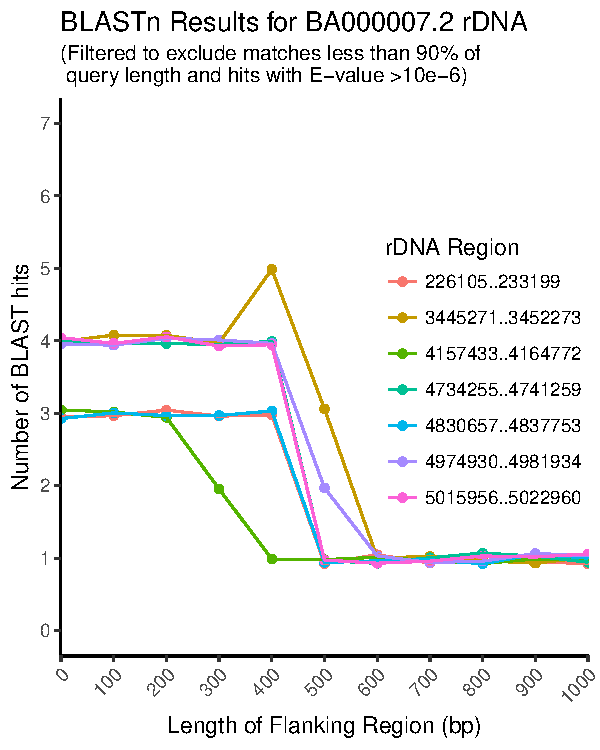
\includegraphics[width=.5\textwidth]{grouped_sakai_BLAST_results}
    \caption{BLASTn was used to perform \textit{in silico} DNA-DNA hybridization of all rDNA regions from \textit{E. coli Sakai} with variable flanking lengths. The number of hits is a proxy for occurrences in the genome; increasing the flanking length increases the specificity. (Points are jittered to aid visibility for overlapping values.)}
    \label{fig:blast}
  \end{figure}

\begin{figure}[H]
    \centering
    \hspace*{0cm}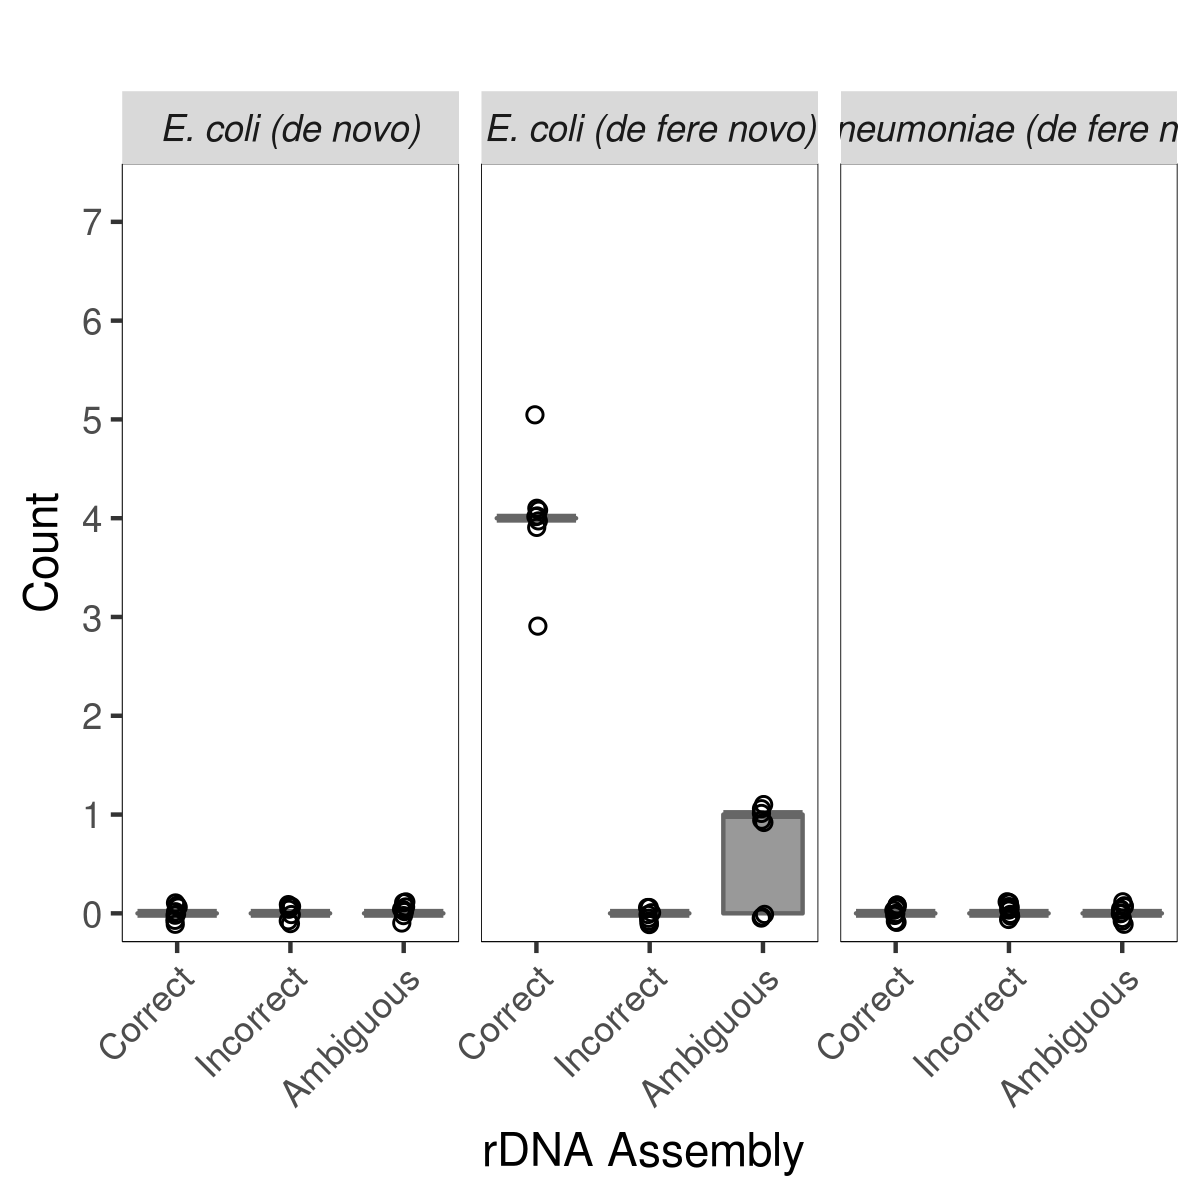
\includegraphics[width=.60\textwidth]{simulated_genome}
    \caption{Assembly of artificial genome. \textit{De fere novo} results in closure of 3-5 rDNAs with the correct reference; only 1-2 rDNAs are correctly assembled using \textit{K. pneumoniae}.  No rDNAs are assembled with \textit{de novo} assembly. Scored with riboScore.py. N=8.}
    \label{fig:simgenome}
\end{figure}


\begin{figure}[H]
  \centering
  \begin{subfigure}[b]{.45\textwidth}
    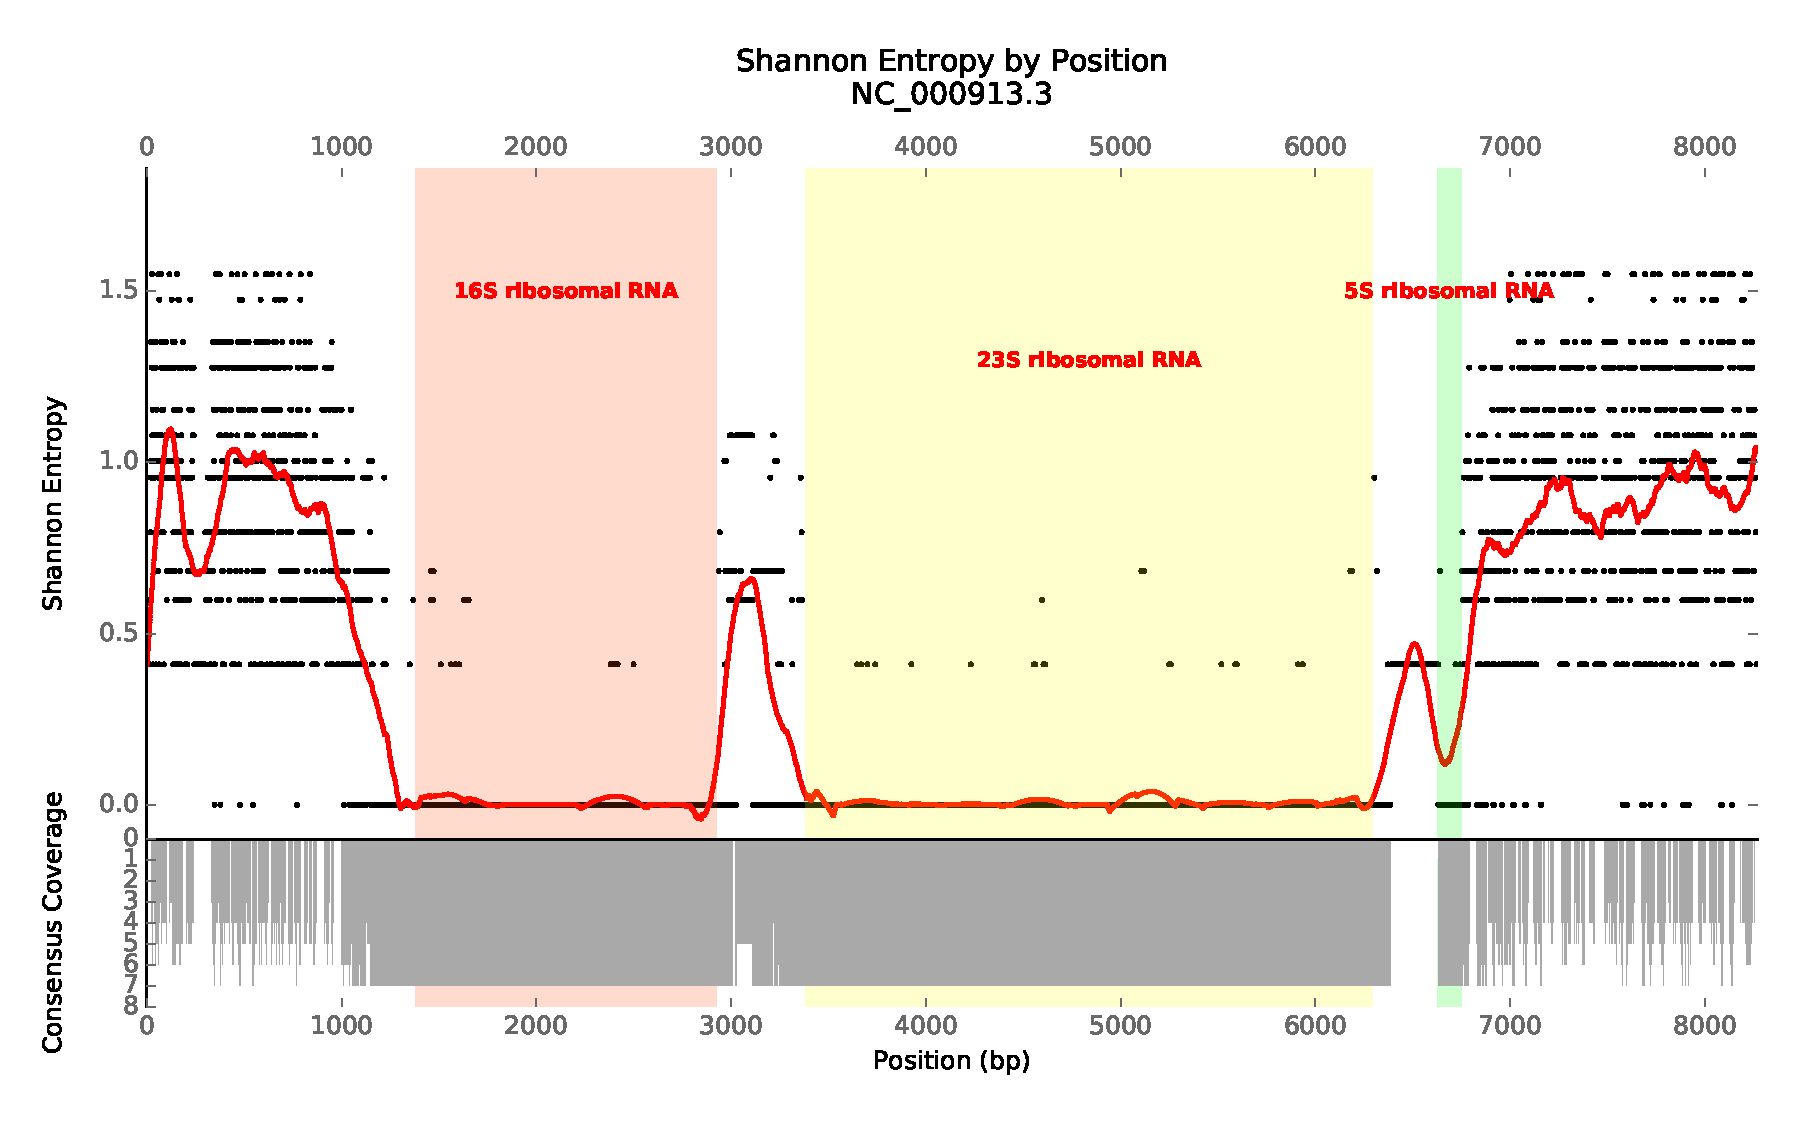
\includegraphics[width=0.95\textwidth]{gage_entropy_figures/NC_000913.3_entropy_plot}
    \caption{\textit{E. coli MG1655} (NC\_000913.3)}
    \label{fig:ent_coli}
  \end{subfigure}
  \begin{subfigure}[b]{.45\textwidth}
    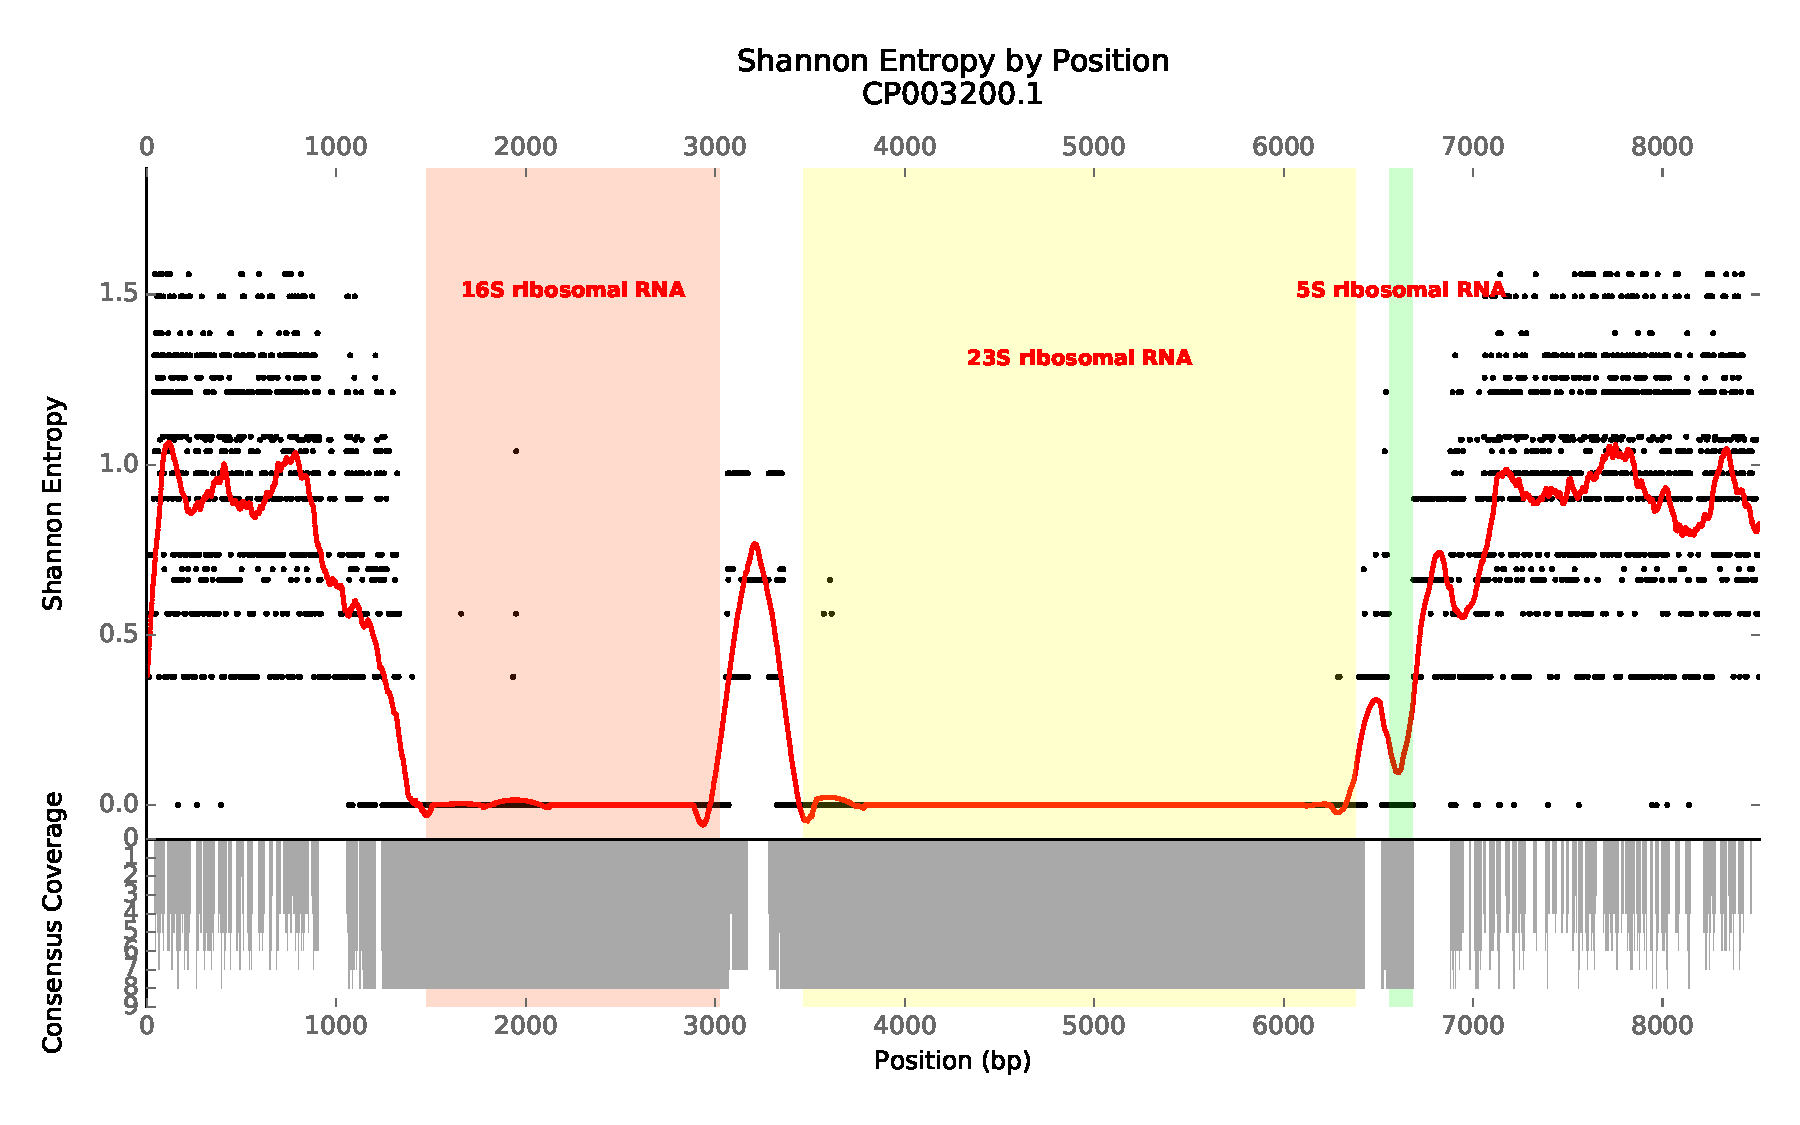
\includegraphics[width=0.95\textwidth]{gage_entropy_figures/CP003200.1_entropy_plot}
    \caption{\textit{K. pneumoniae subsp. pneumoniae HS11286} (CP003200.1) }
    \label{fig:ent_pneumo}
  \end{subfigure}
  \begin{subfigure}[b]{.45\textwidth}
    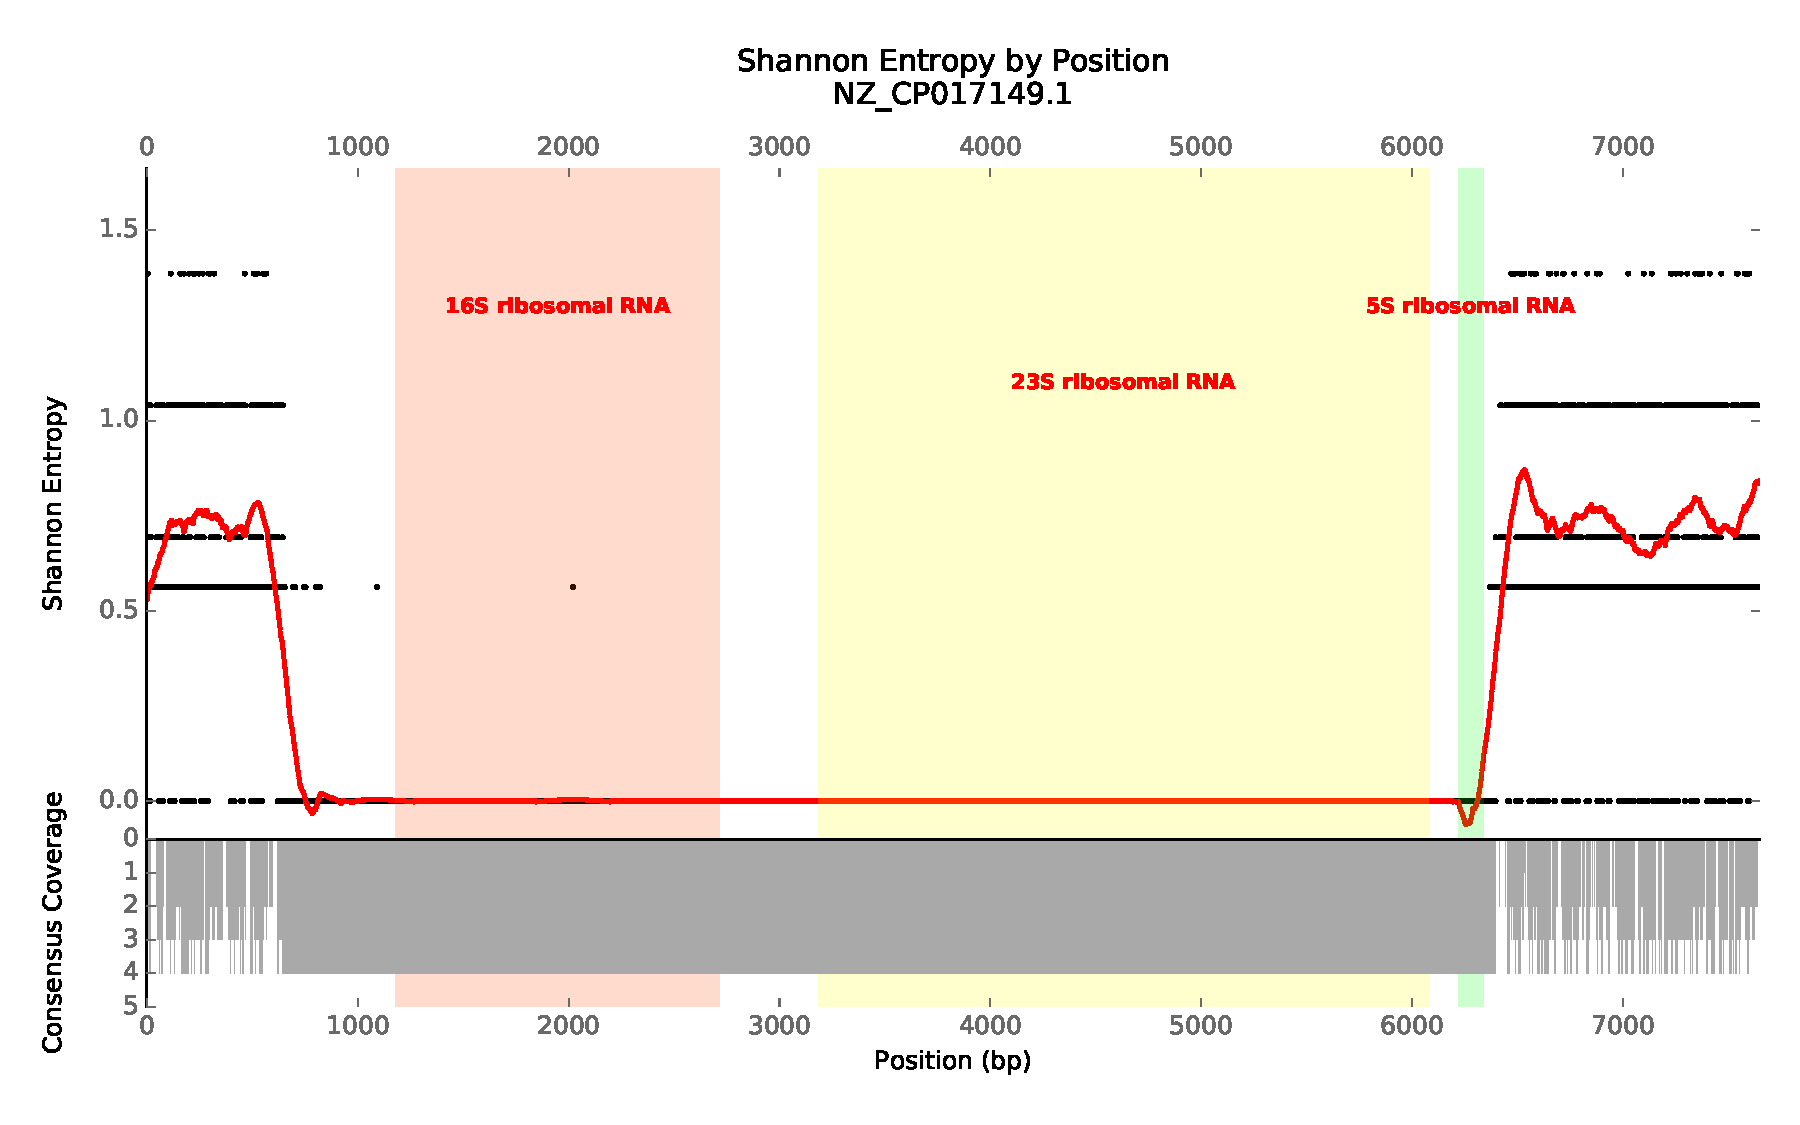
\includegraphics[width=0.95\textwidth]{gage_entropy_figures/NZ_CP017149.1_entropy_plot}
    \caption{\textit{P. aeruginosa strain ATCC 15692} (NZ\_CP017149.1)}
    \label{fig:ent_pao}
  \end{subfigure}
  \begin{subfigure}[b]{.45\textwidth}
    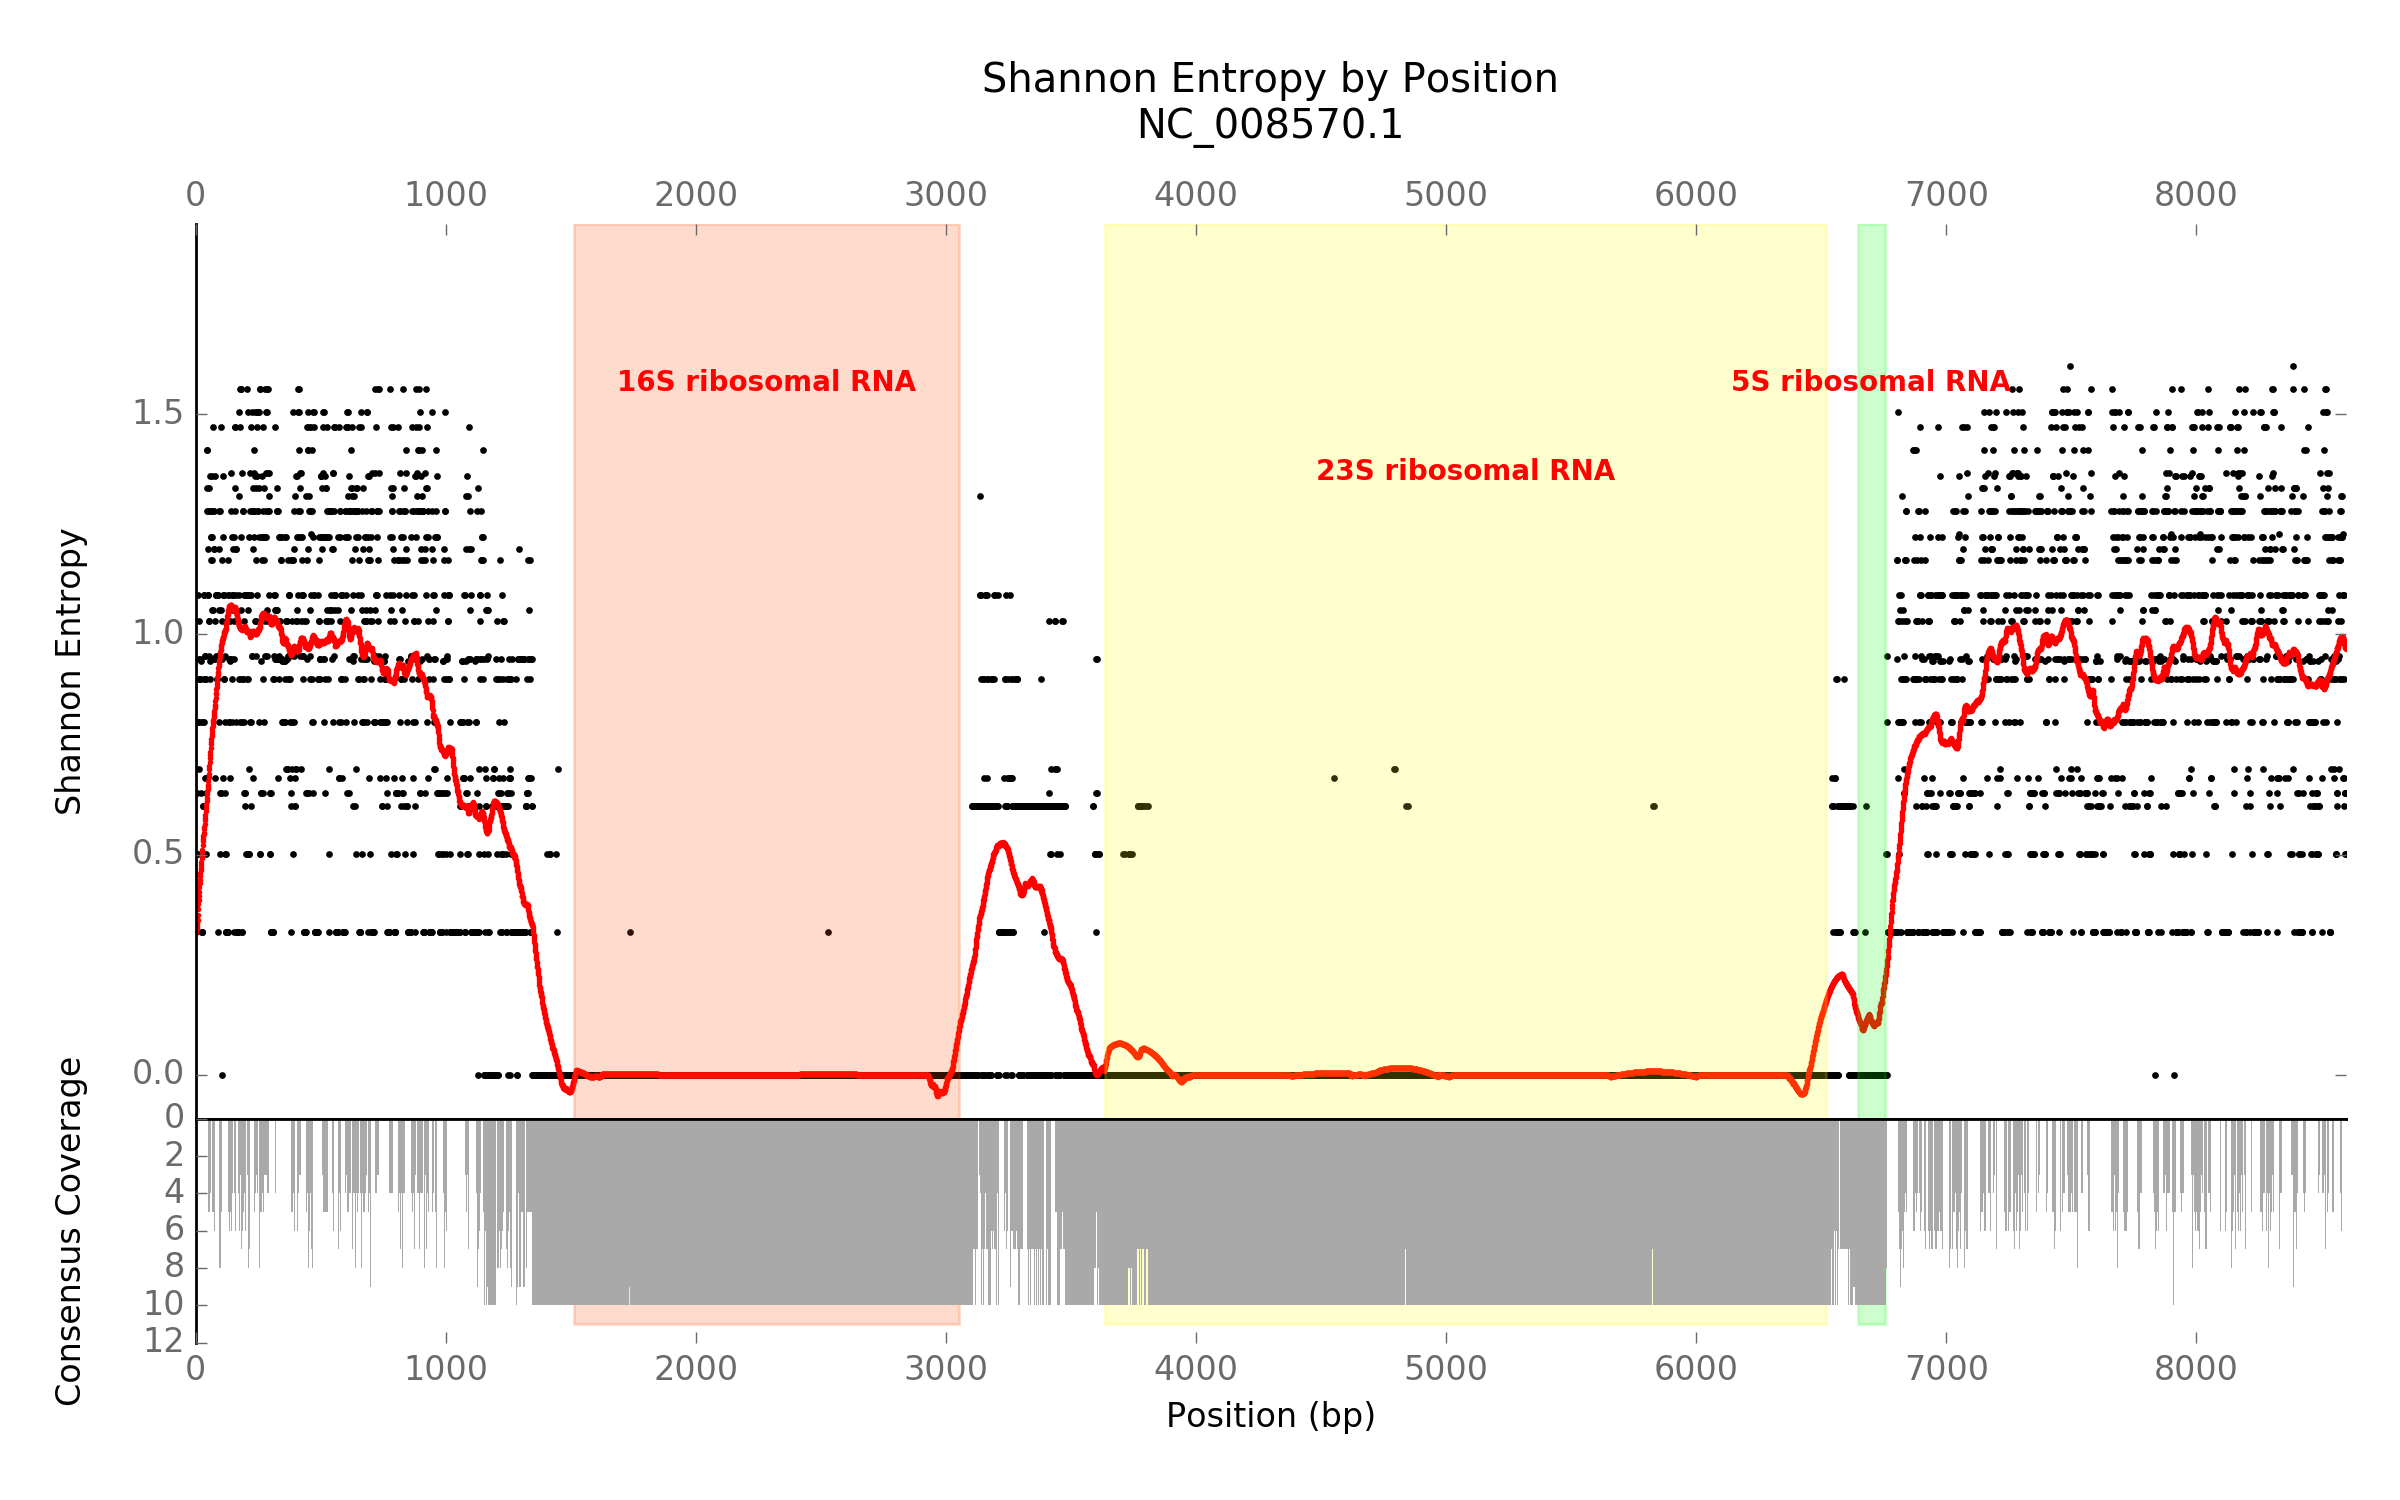
\includegraphics[width=0.95\textwidth]{gage_entropy_figures/NC_008570.1_entropy_plot}
    \caption{\textit{A. hydrophila ATCC 7966} (NC\_008570.1)}
    \label{fig:ent_aero}
  \end{subfigure}
  \begin{subfigure}[b]{.45\textwidth}
    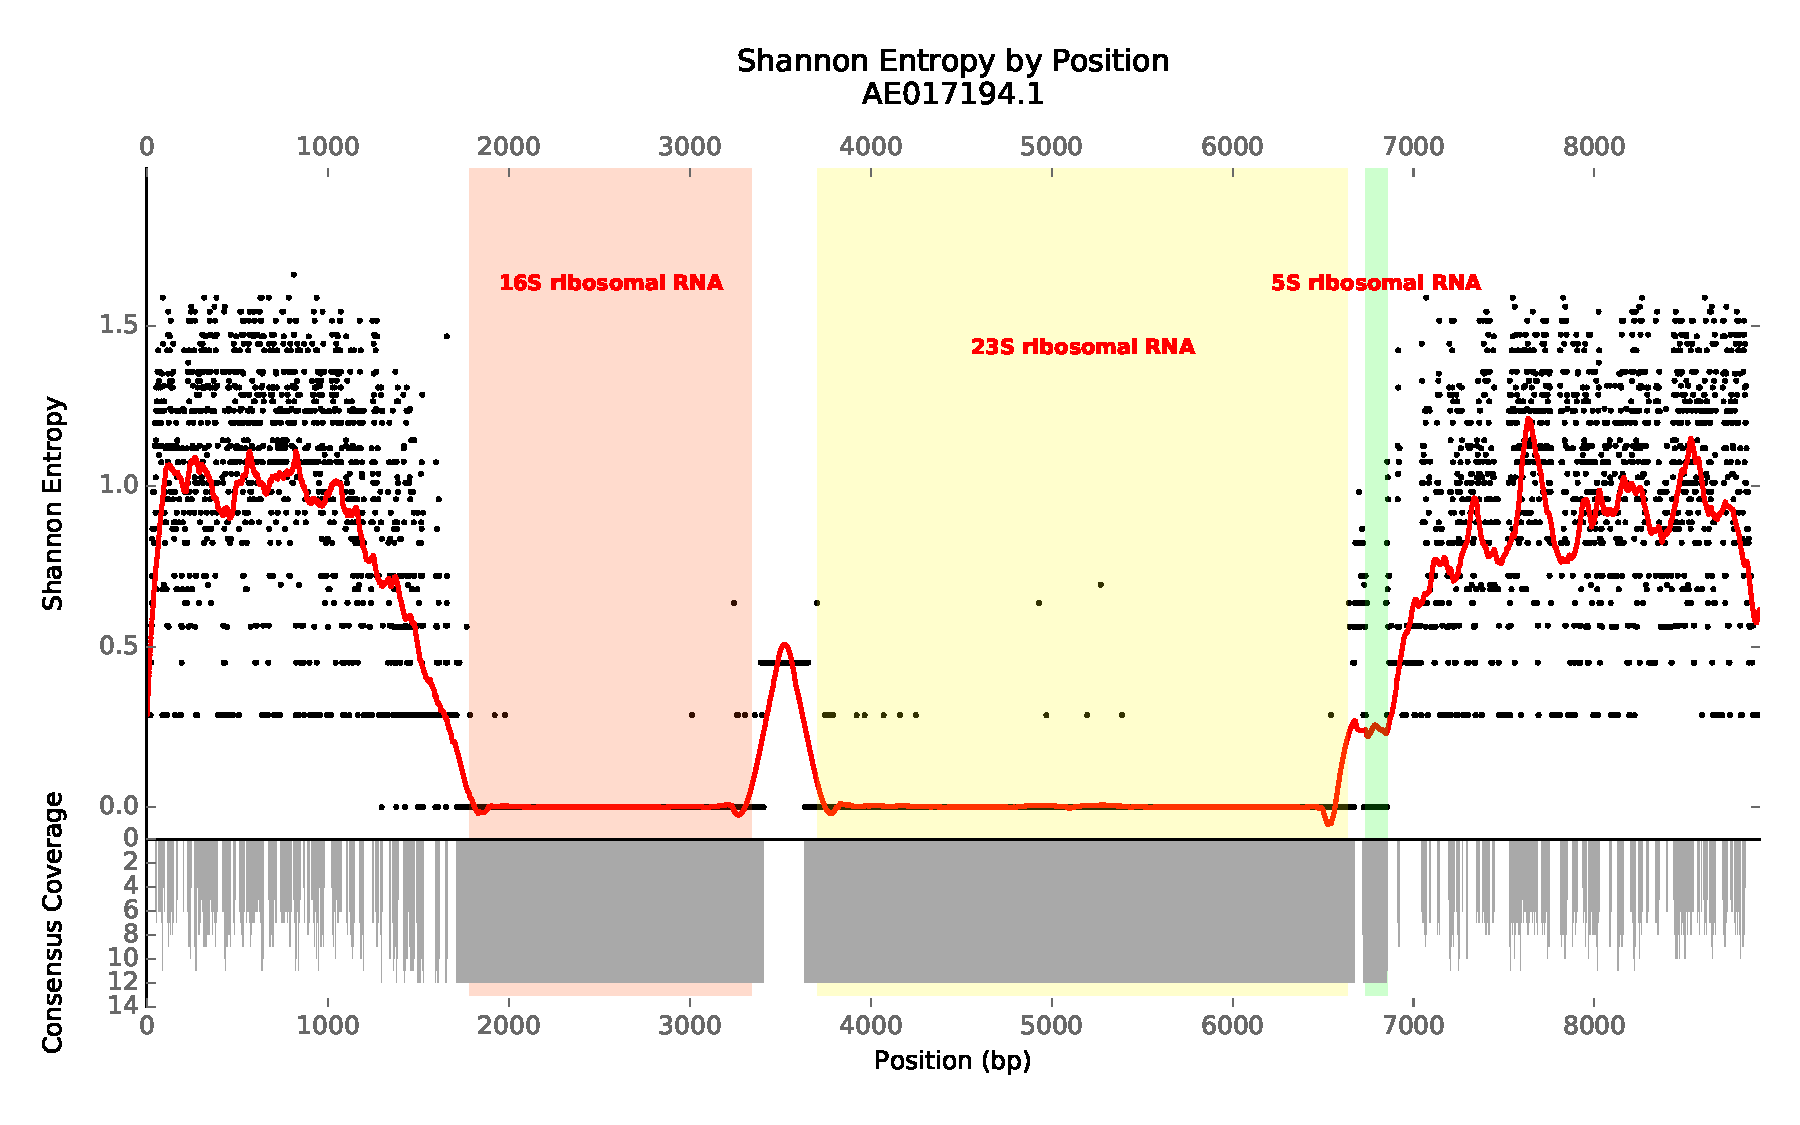
\includegraphics[width=0.95\textwidth]{gage_entropy_figures/AE017194.1_entropy_plot}
    \caption{\textit{B. cereus ATCC 10987} (AE017194.1)}
    \label{fig:ent_cereus_atcc}
  \end{subfigure}
  \begin{subfigure}[b]{.45\textwidth}
    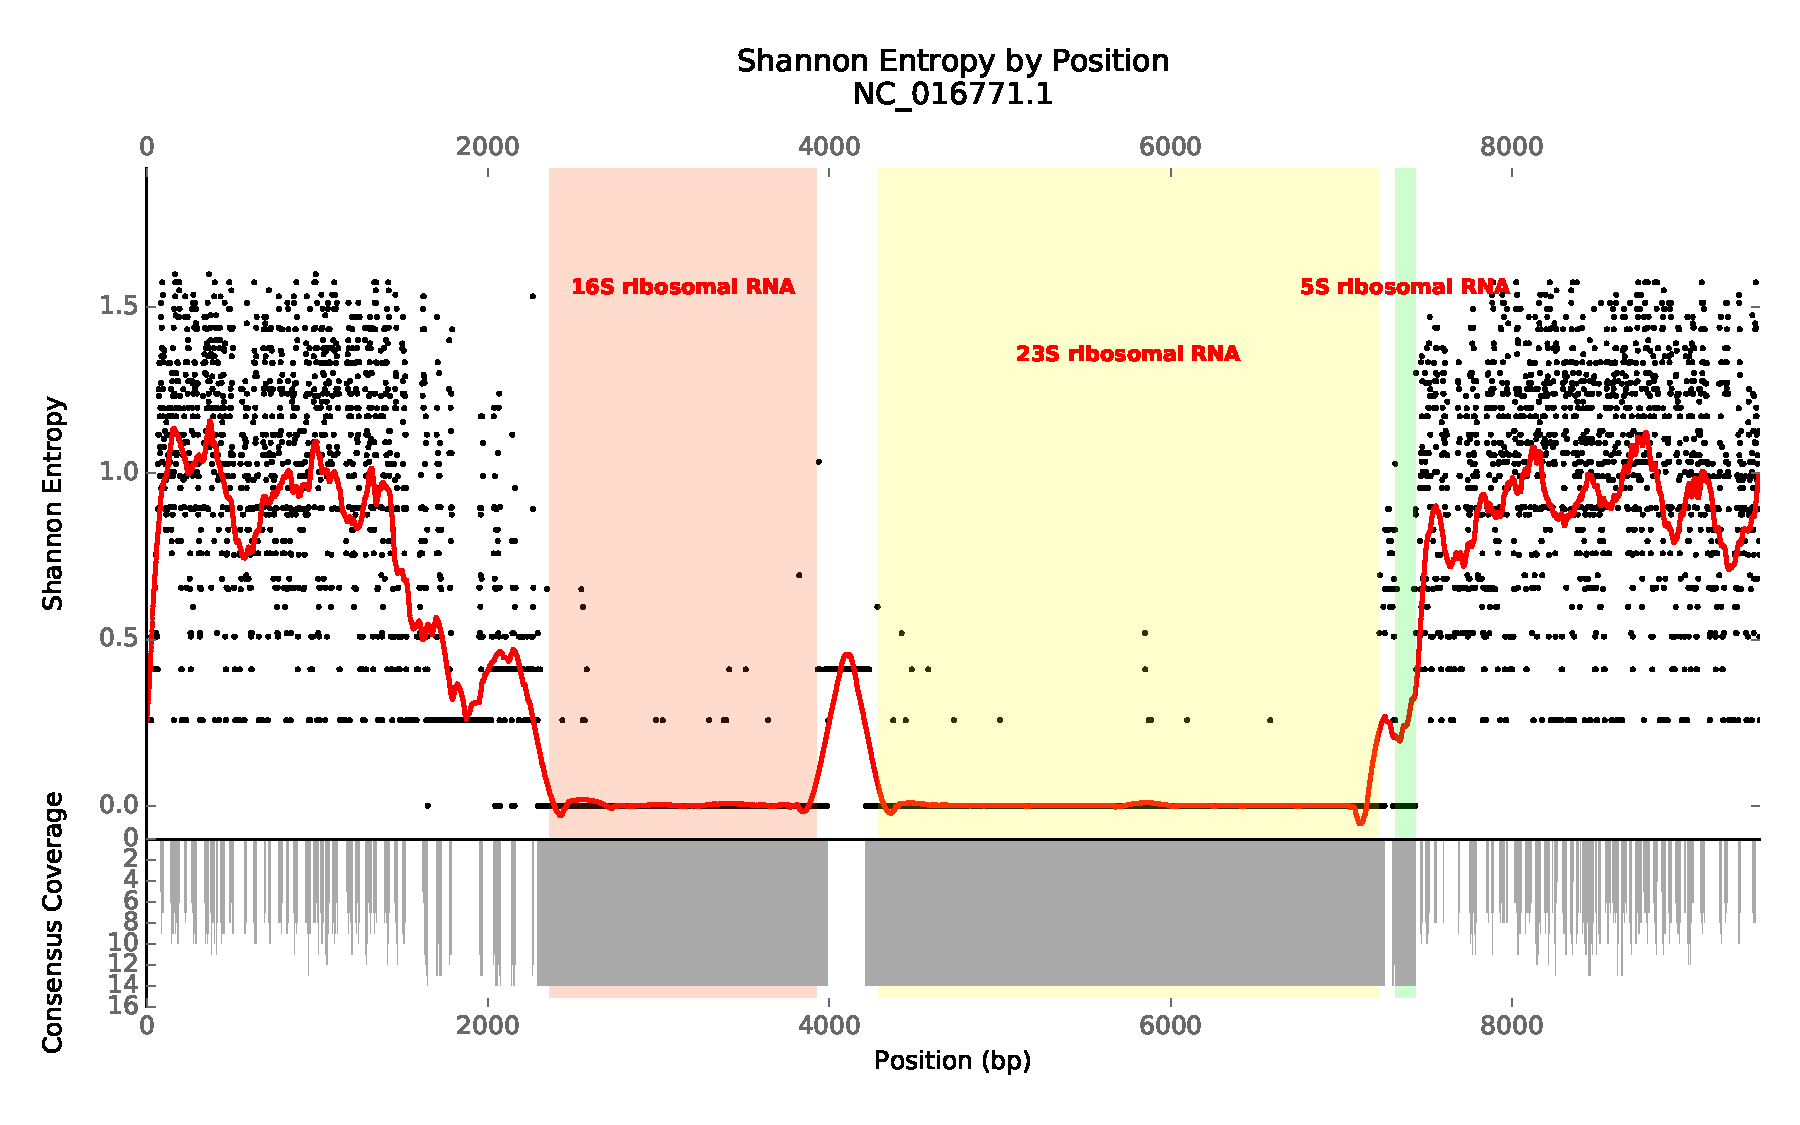
\includegraphics[width=0.95\textwidth]{gage_entropy_figures/NC_016771.1_entropy_plot}
    \caption{\textit{B. cereus NC7401} (NC\_016771.1)}
    \label{fig:ent_cereus_nc}
  \end{subfigure}
  \begin{subfigure}[b]{.45\textwidth}
    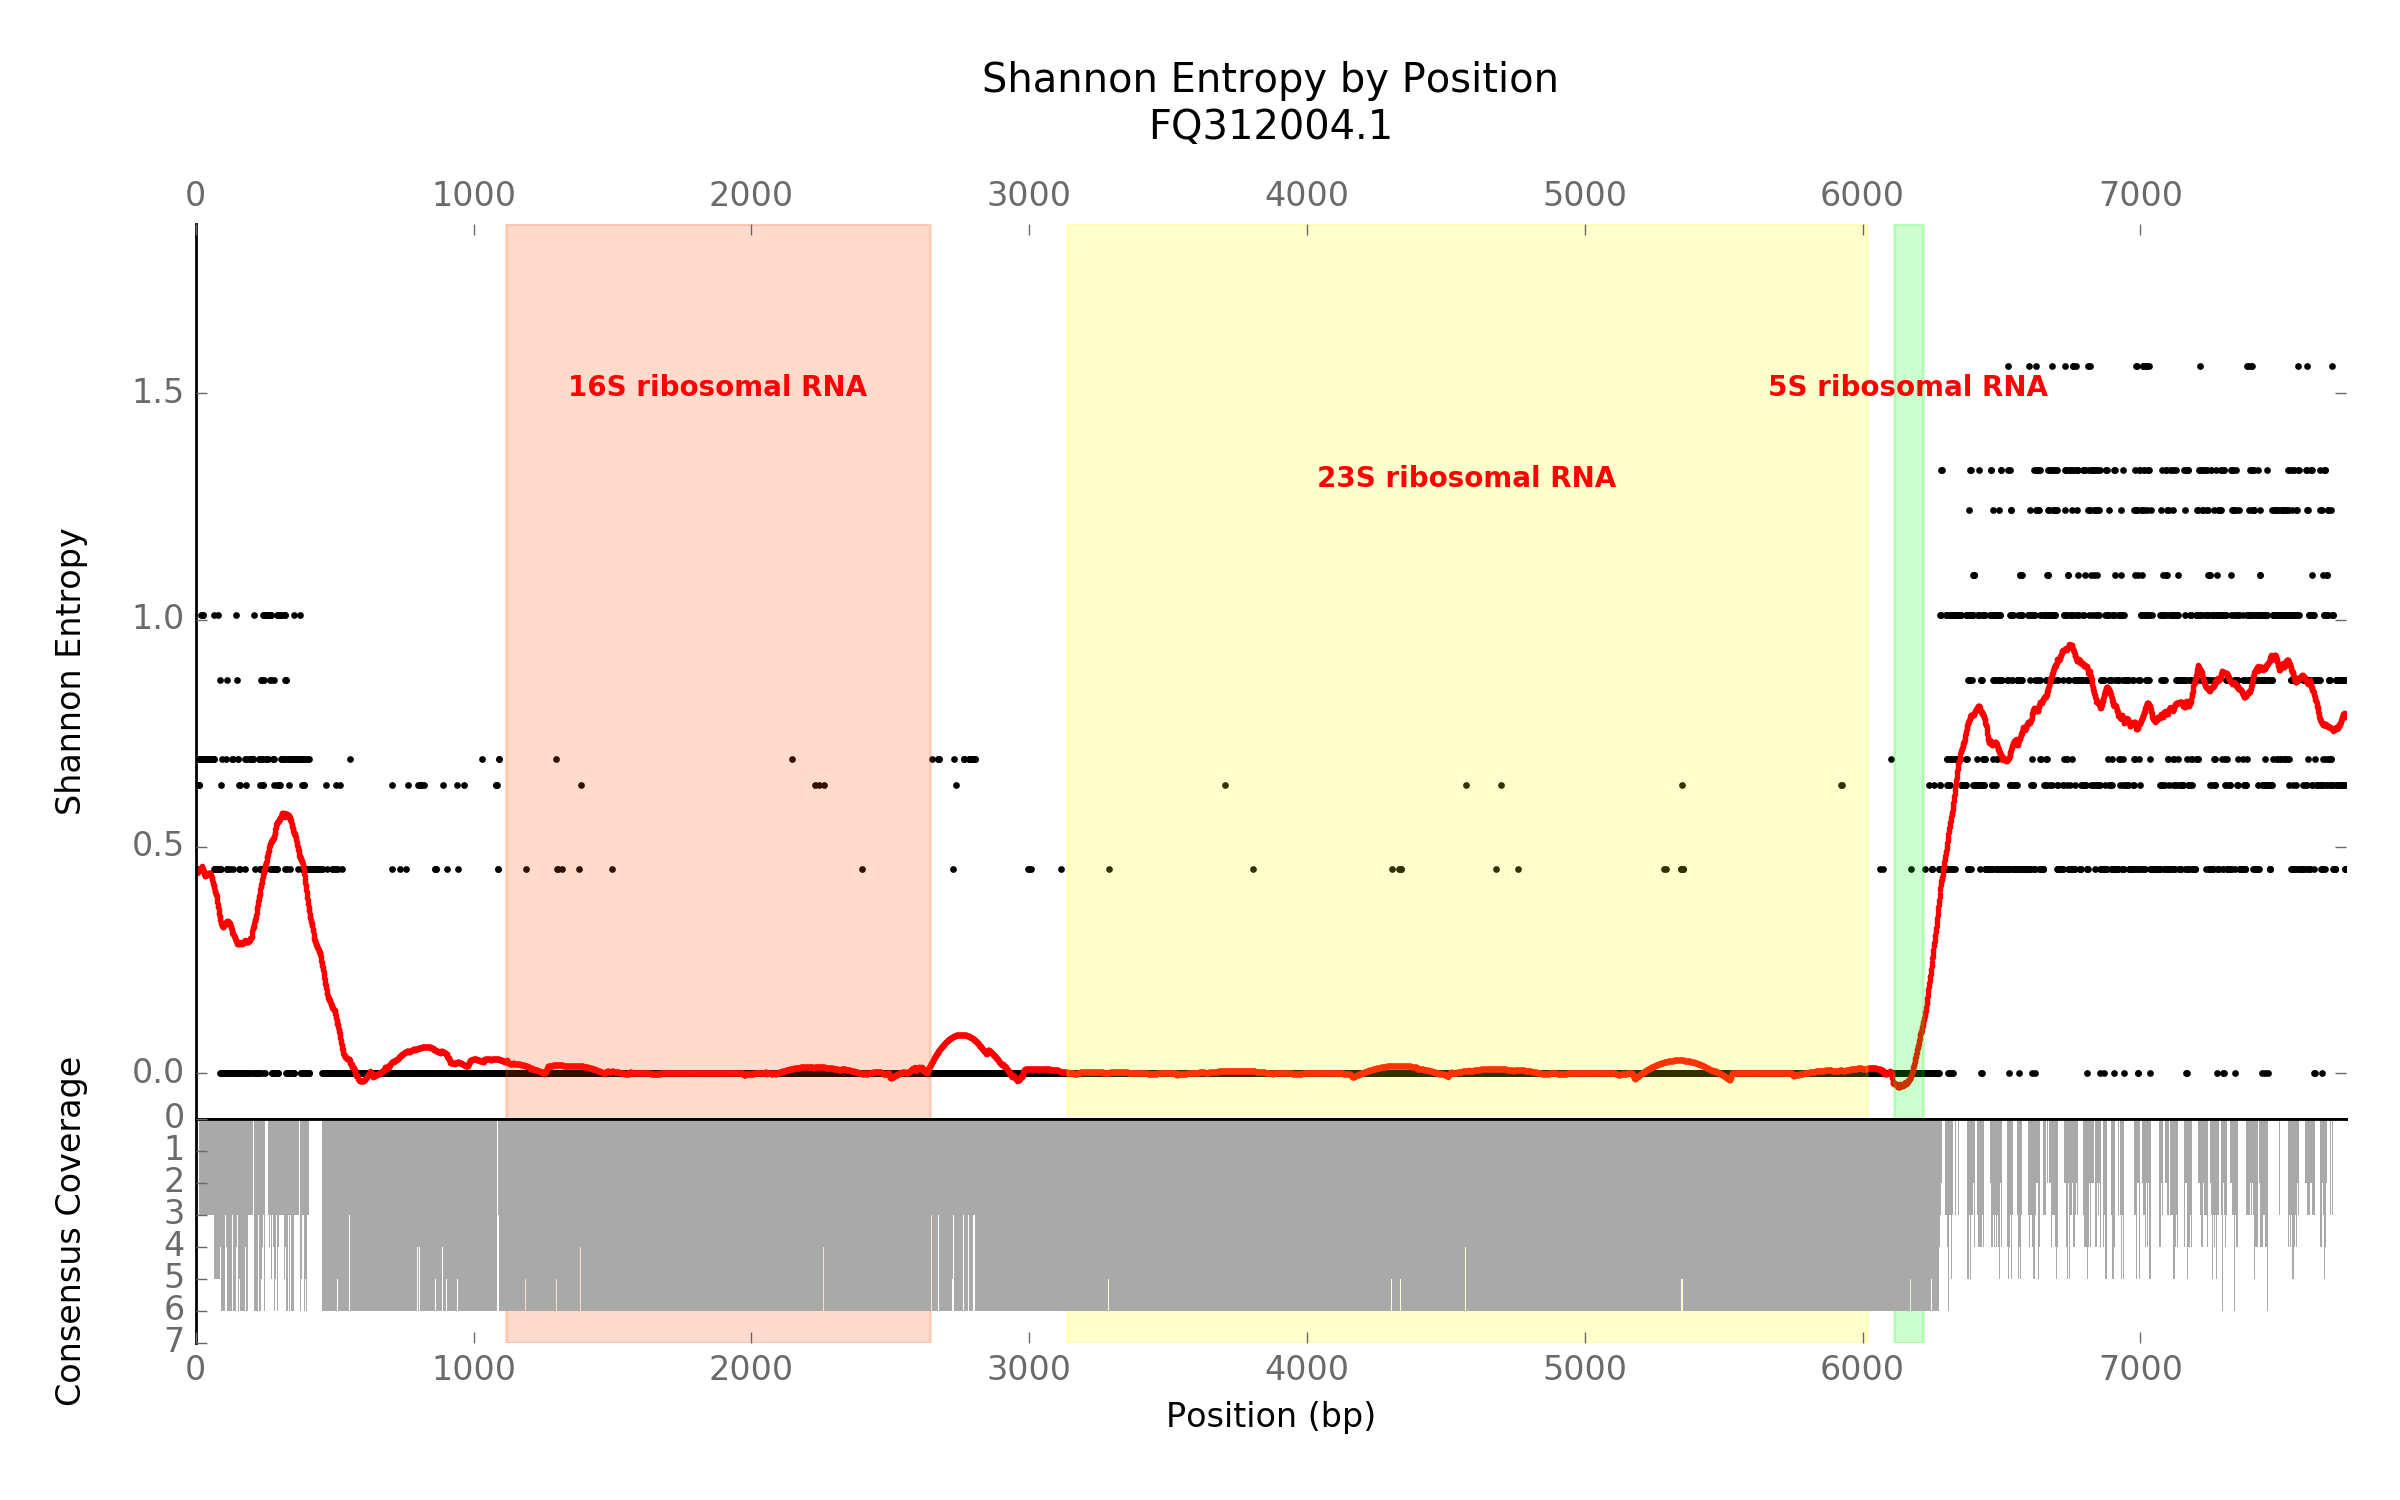
\includegraphics[width=0.95\textwidth]{gage_entropy_figures/FQ312004.1_entropy_plot}
    \caption{\textit{B. fragilis 638R} (FQ312004.1)}
    \label{fig:ent_frag}
  \end{subfigure}
  \begin{subfigure}[b]{.45\textwidth}
    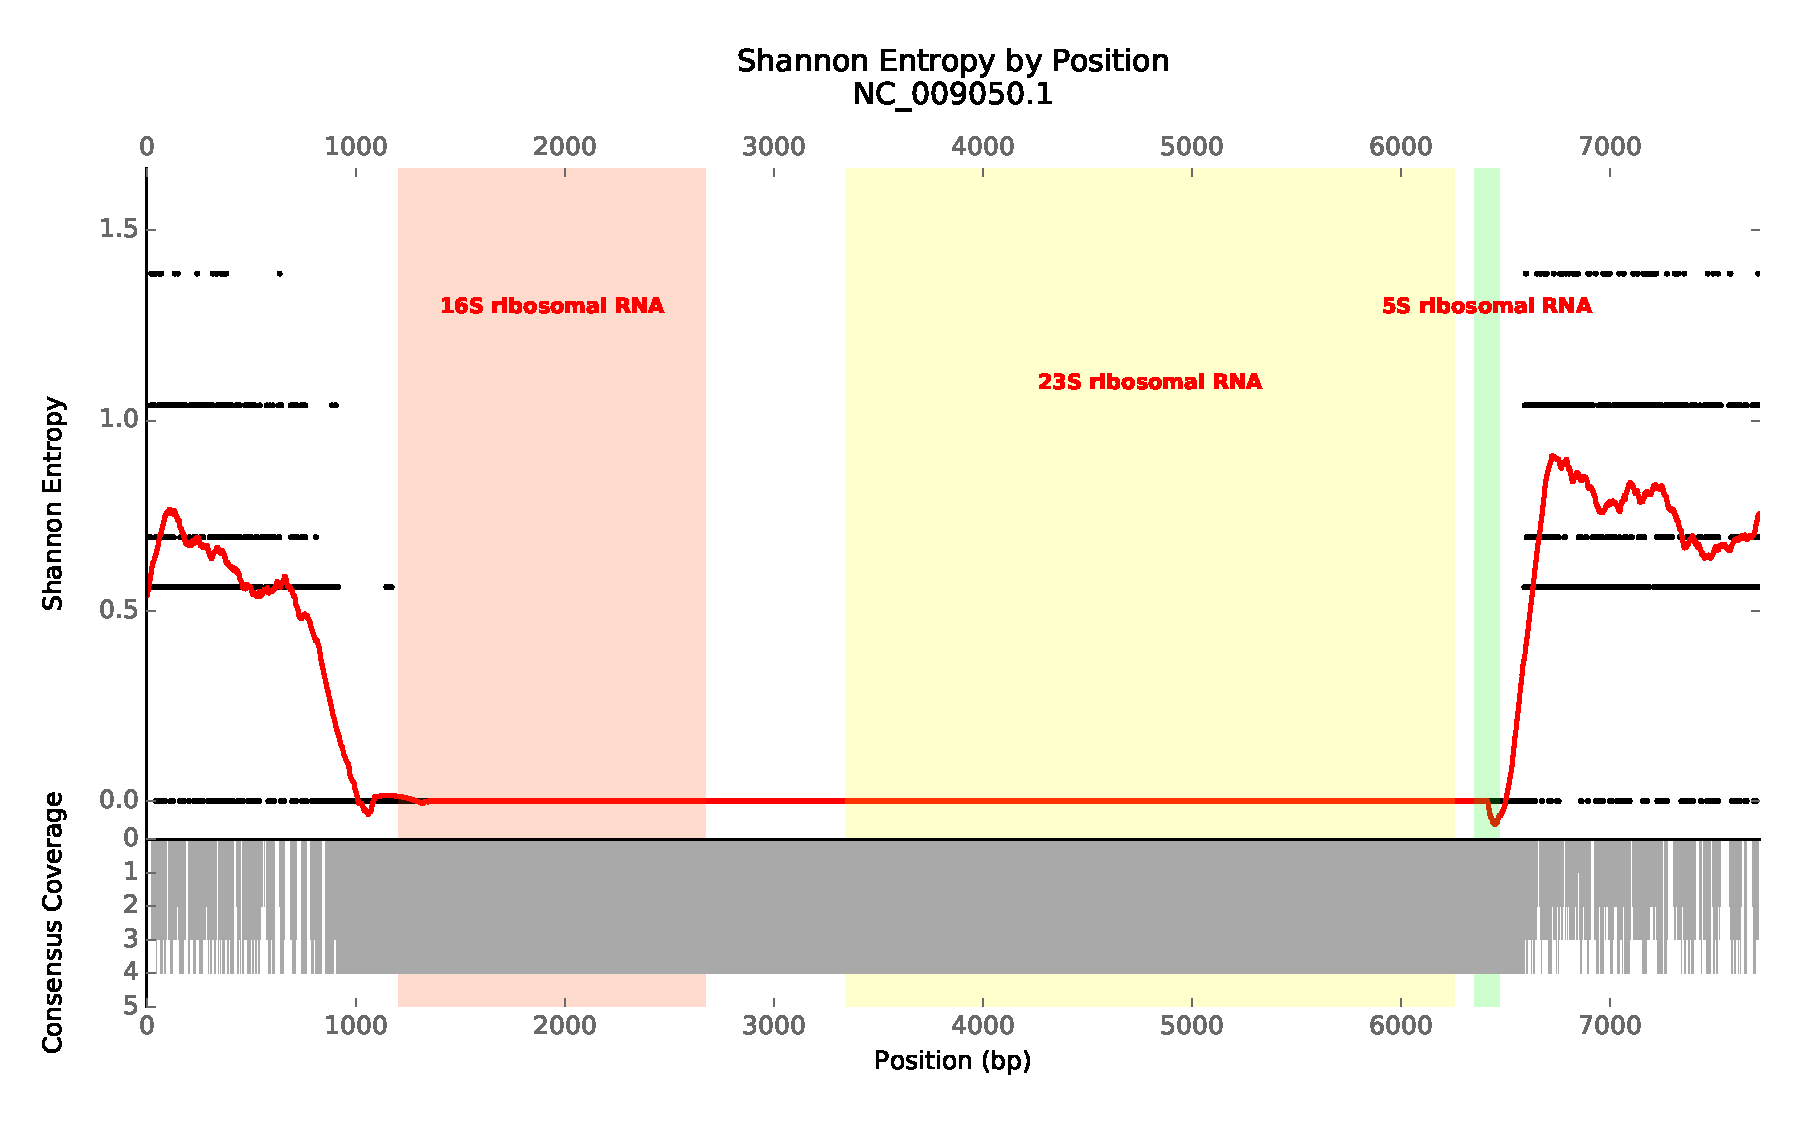
\includegraphics[width=0.95\textwidth]{gage_entropy_figures/NC_009050.1_entropy_plot}
    \caption{\textit{R. sphaeroides  ATCC 17029} (NC\_009049.1, NC\_009050.1)}
    \label{fig:ent_rhodo}
  \end{subfigure}
\end{figure}
\begin{figure}
  \centering
  \ContinuedFloat
  \begin{subfigure}[b]{.45\textwidth}
    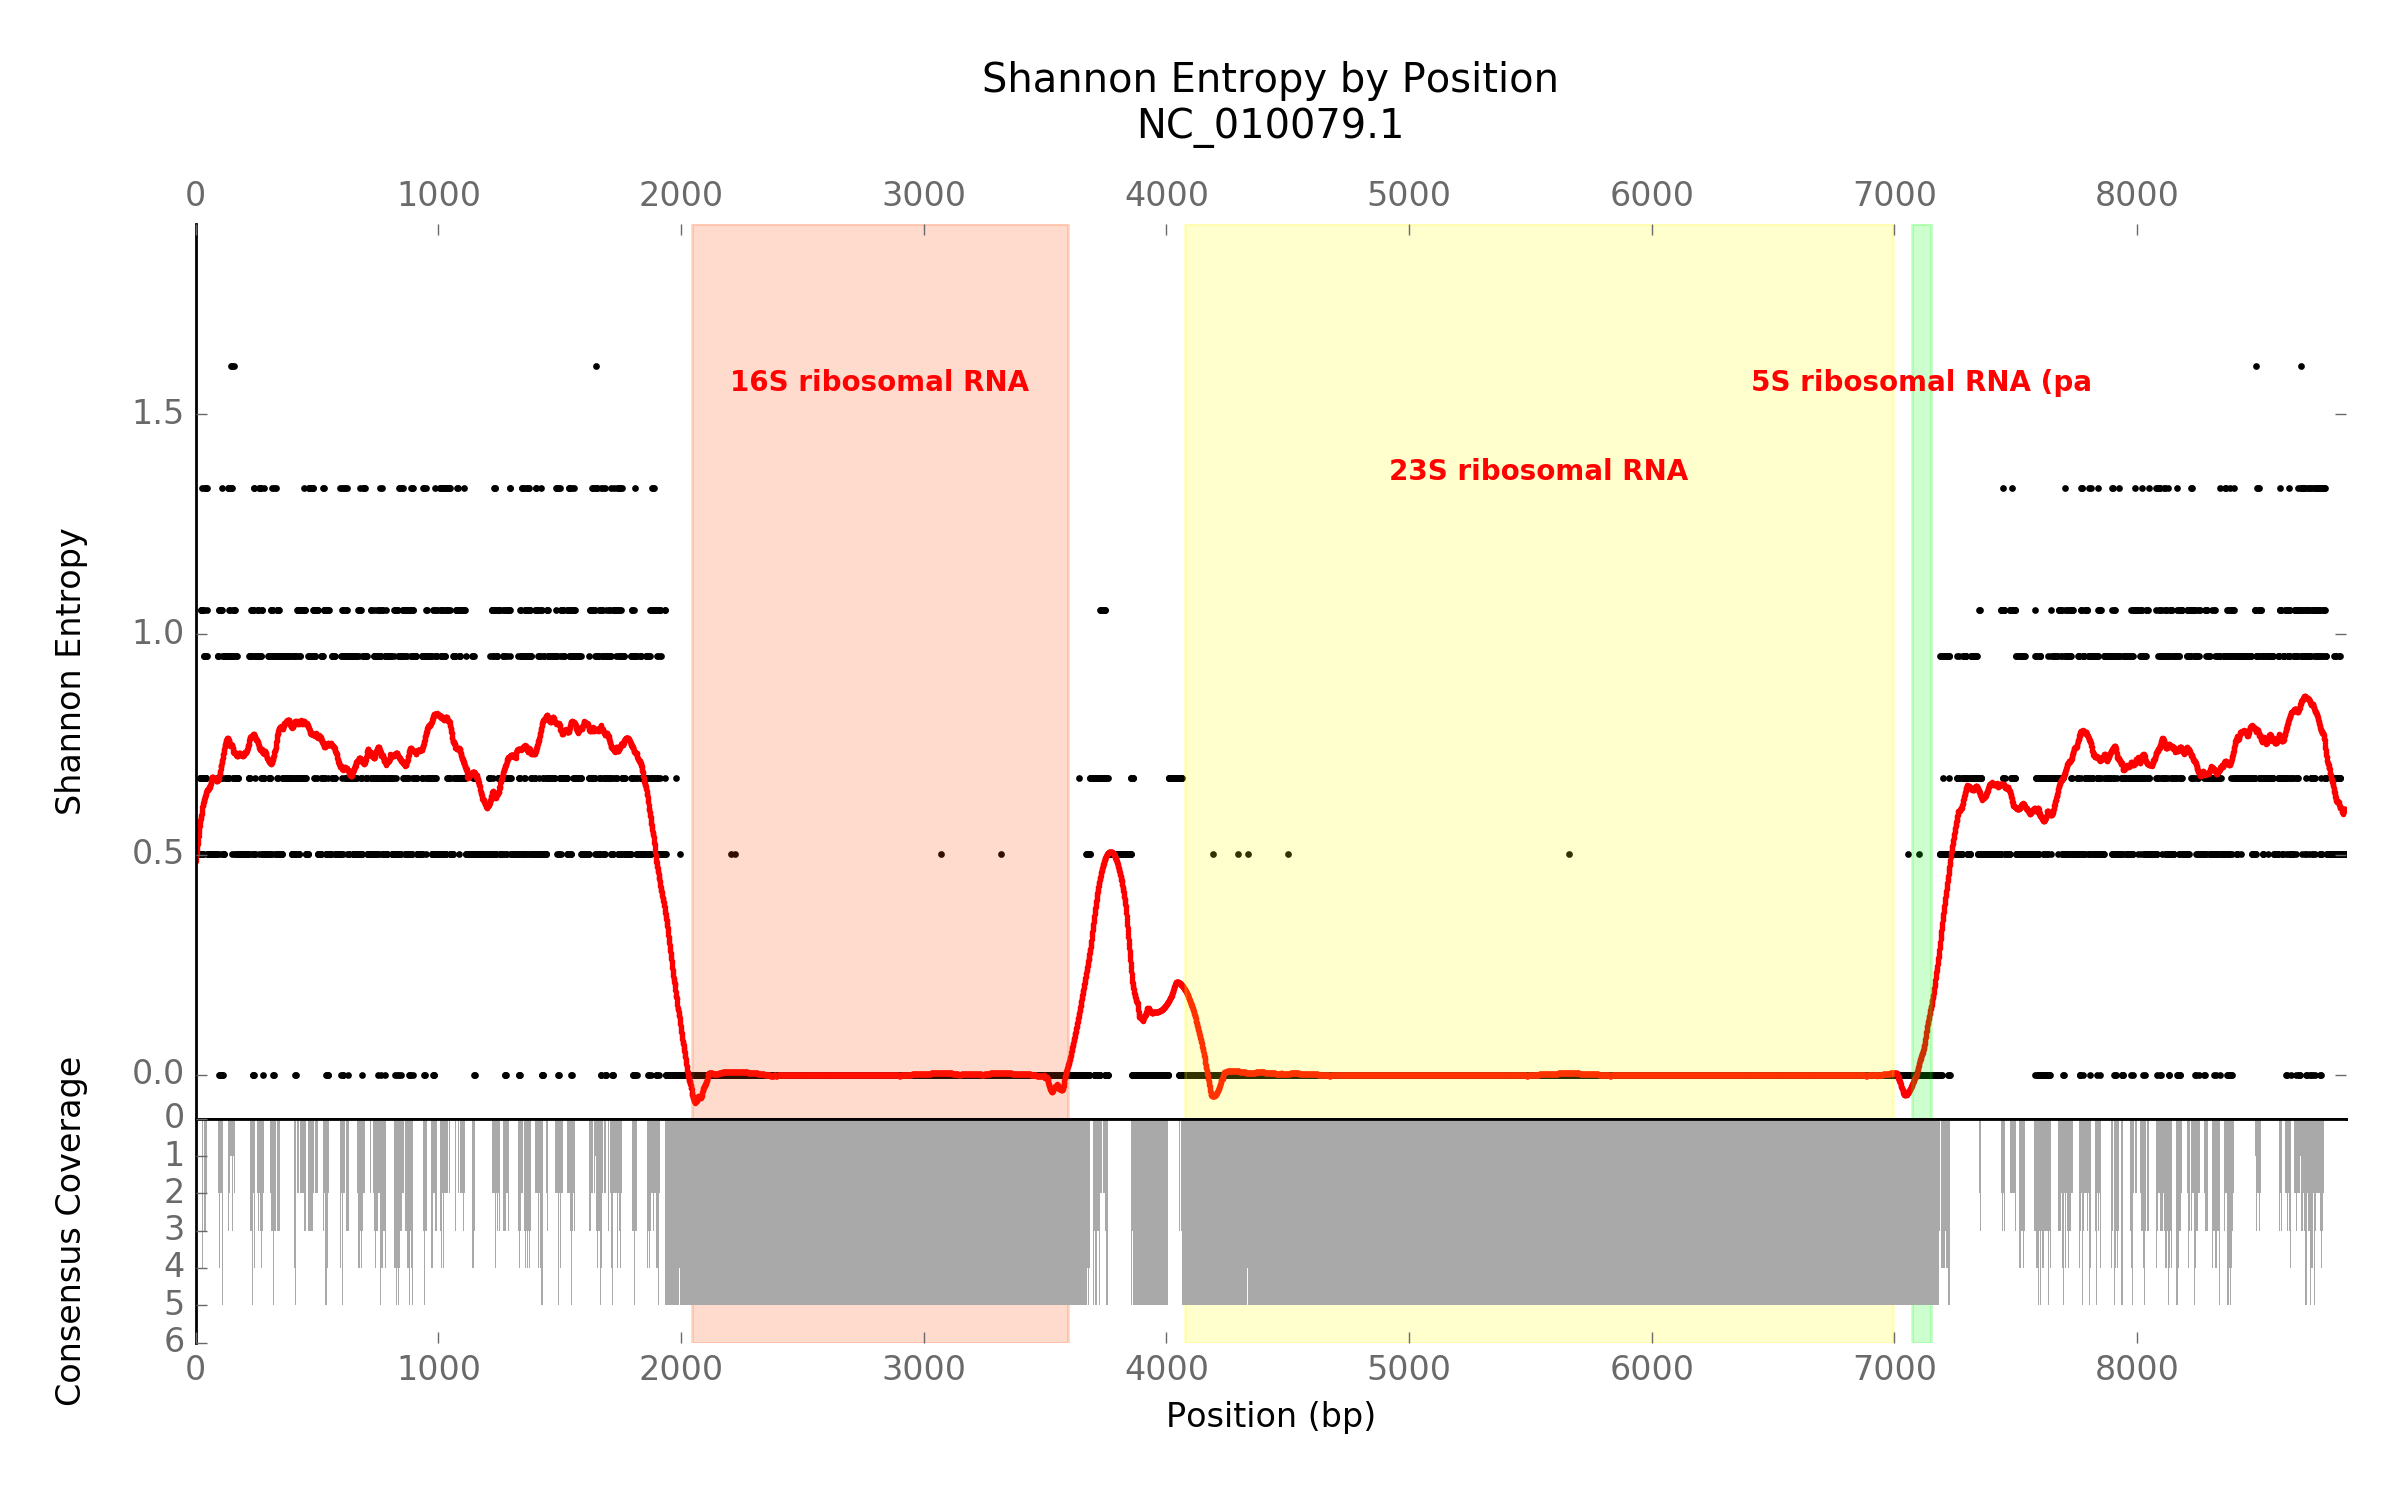
\includegraphics[width=0.95\textwidth]{gage_entropy_figures/NC_010079.1_entropy_plot}
    \caption{\textit{S. aureus TCH1516} (NC\_010079.1)}
    \label{fig:ent_tch}
  \end{subfigure}
  % \begin{subfigure}[b]{.45\textwidth}
  %   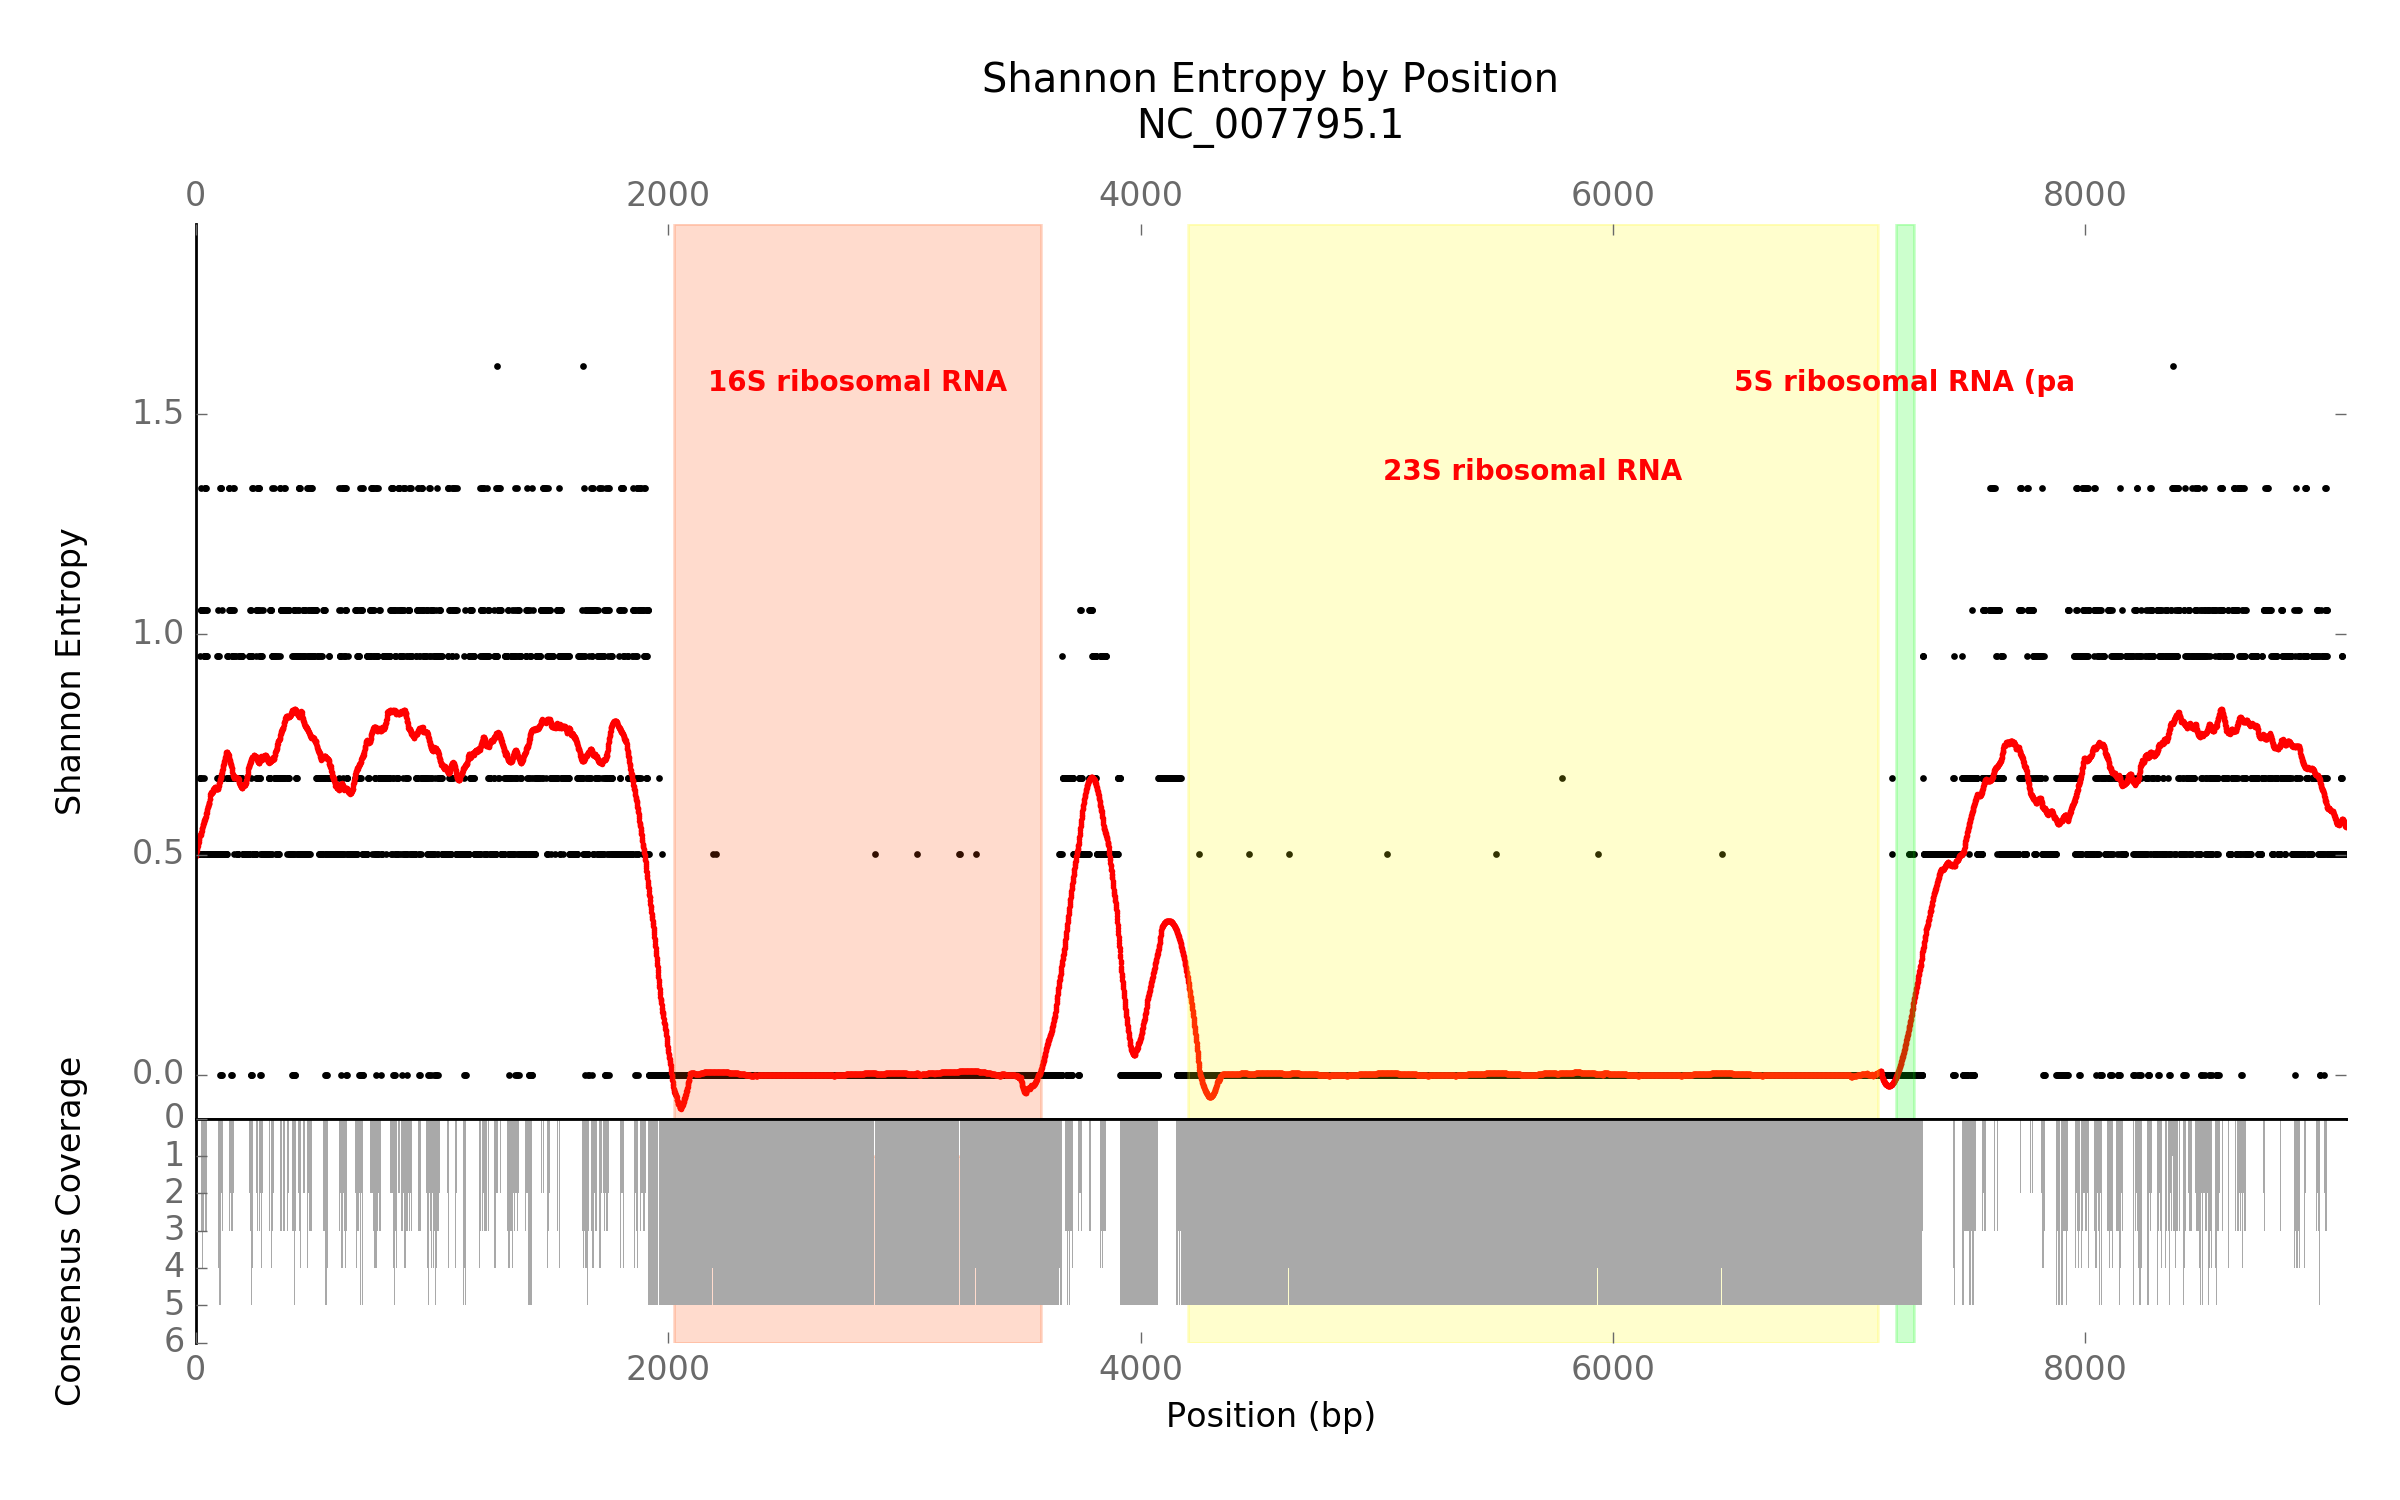
\includegraphics[width=0.95\textwidth]{gage_entropy_figures/NC_007795.1_entropy_plot}
  %   \caption{\textit{S. aureus NCTC 8325} (NC\_007795.1)}
  %   \label{fig:ent_nctc}
  % \end{subfigure}
  % \begin{subfigure}[b]{.45\textwidth}
  %   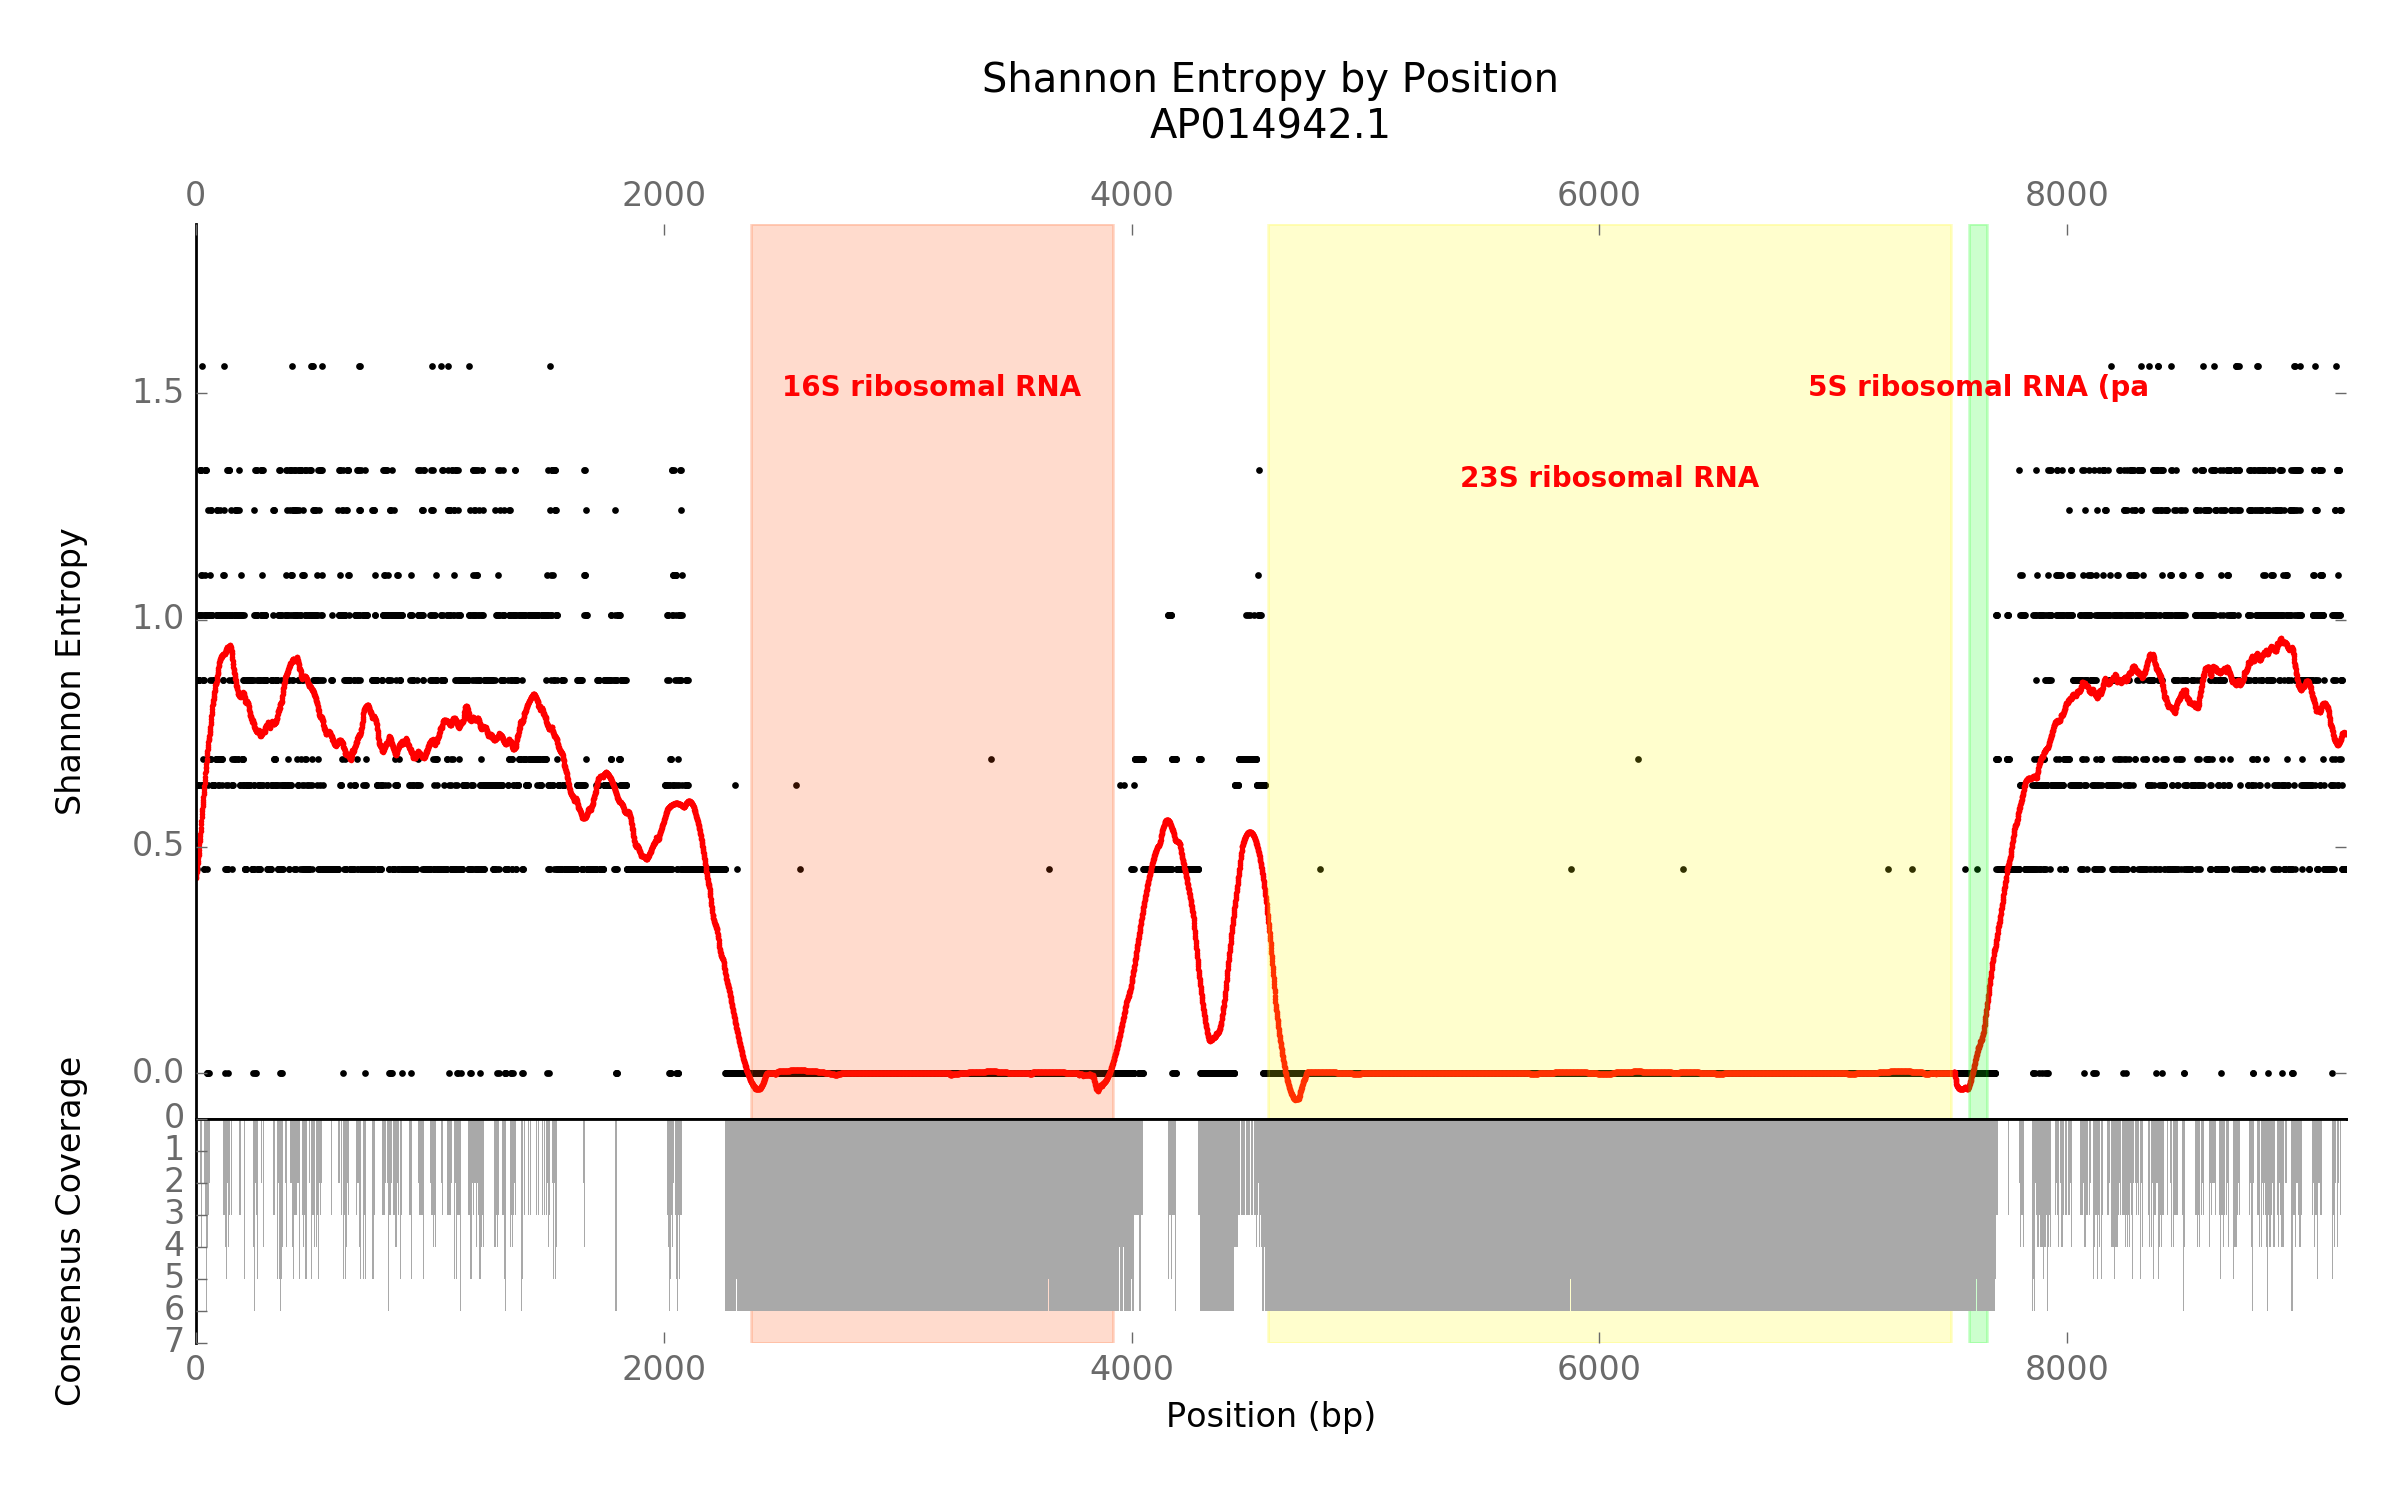
\includegraphics[width=0.95\textwidth]{gage_entropy_figures/AP014942.1_entropy_plot}
  % \caption{\textit{S. aureus FDA209P} (AP014942.1)}
  % \label{fig:entfda}
  % \end{subfigure}
  \begin{subfigure}[b]{.45\textwidth}
    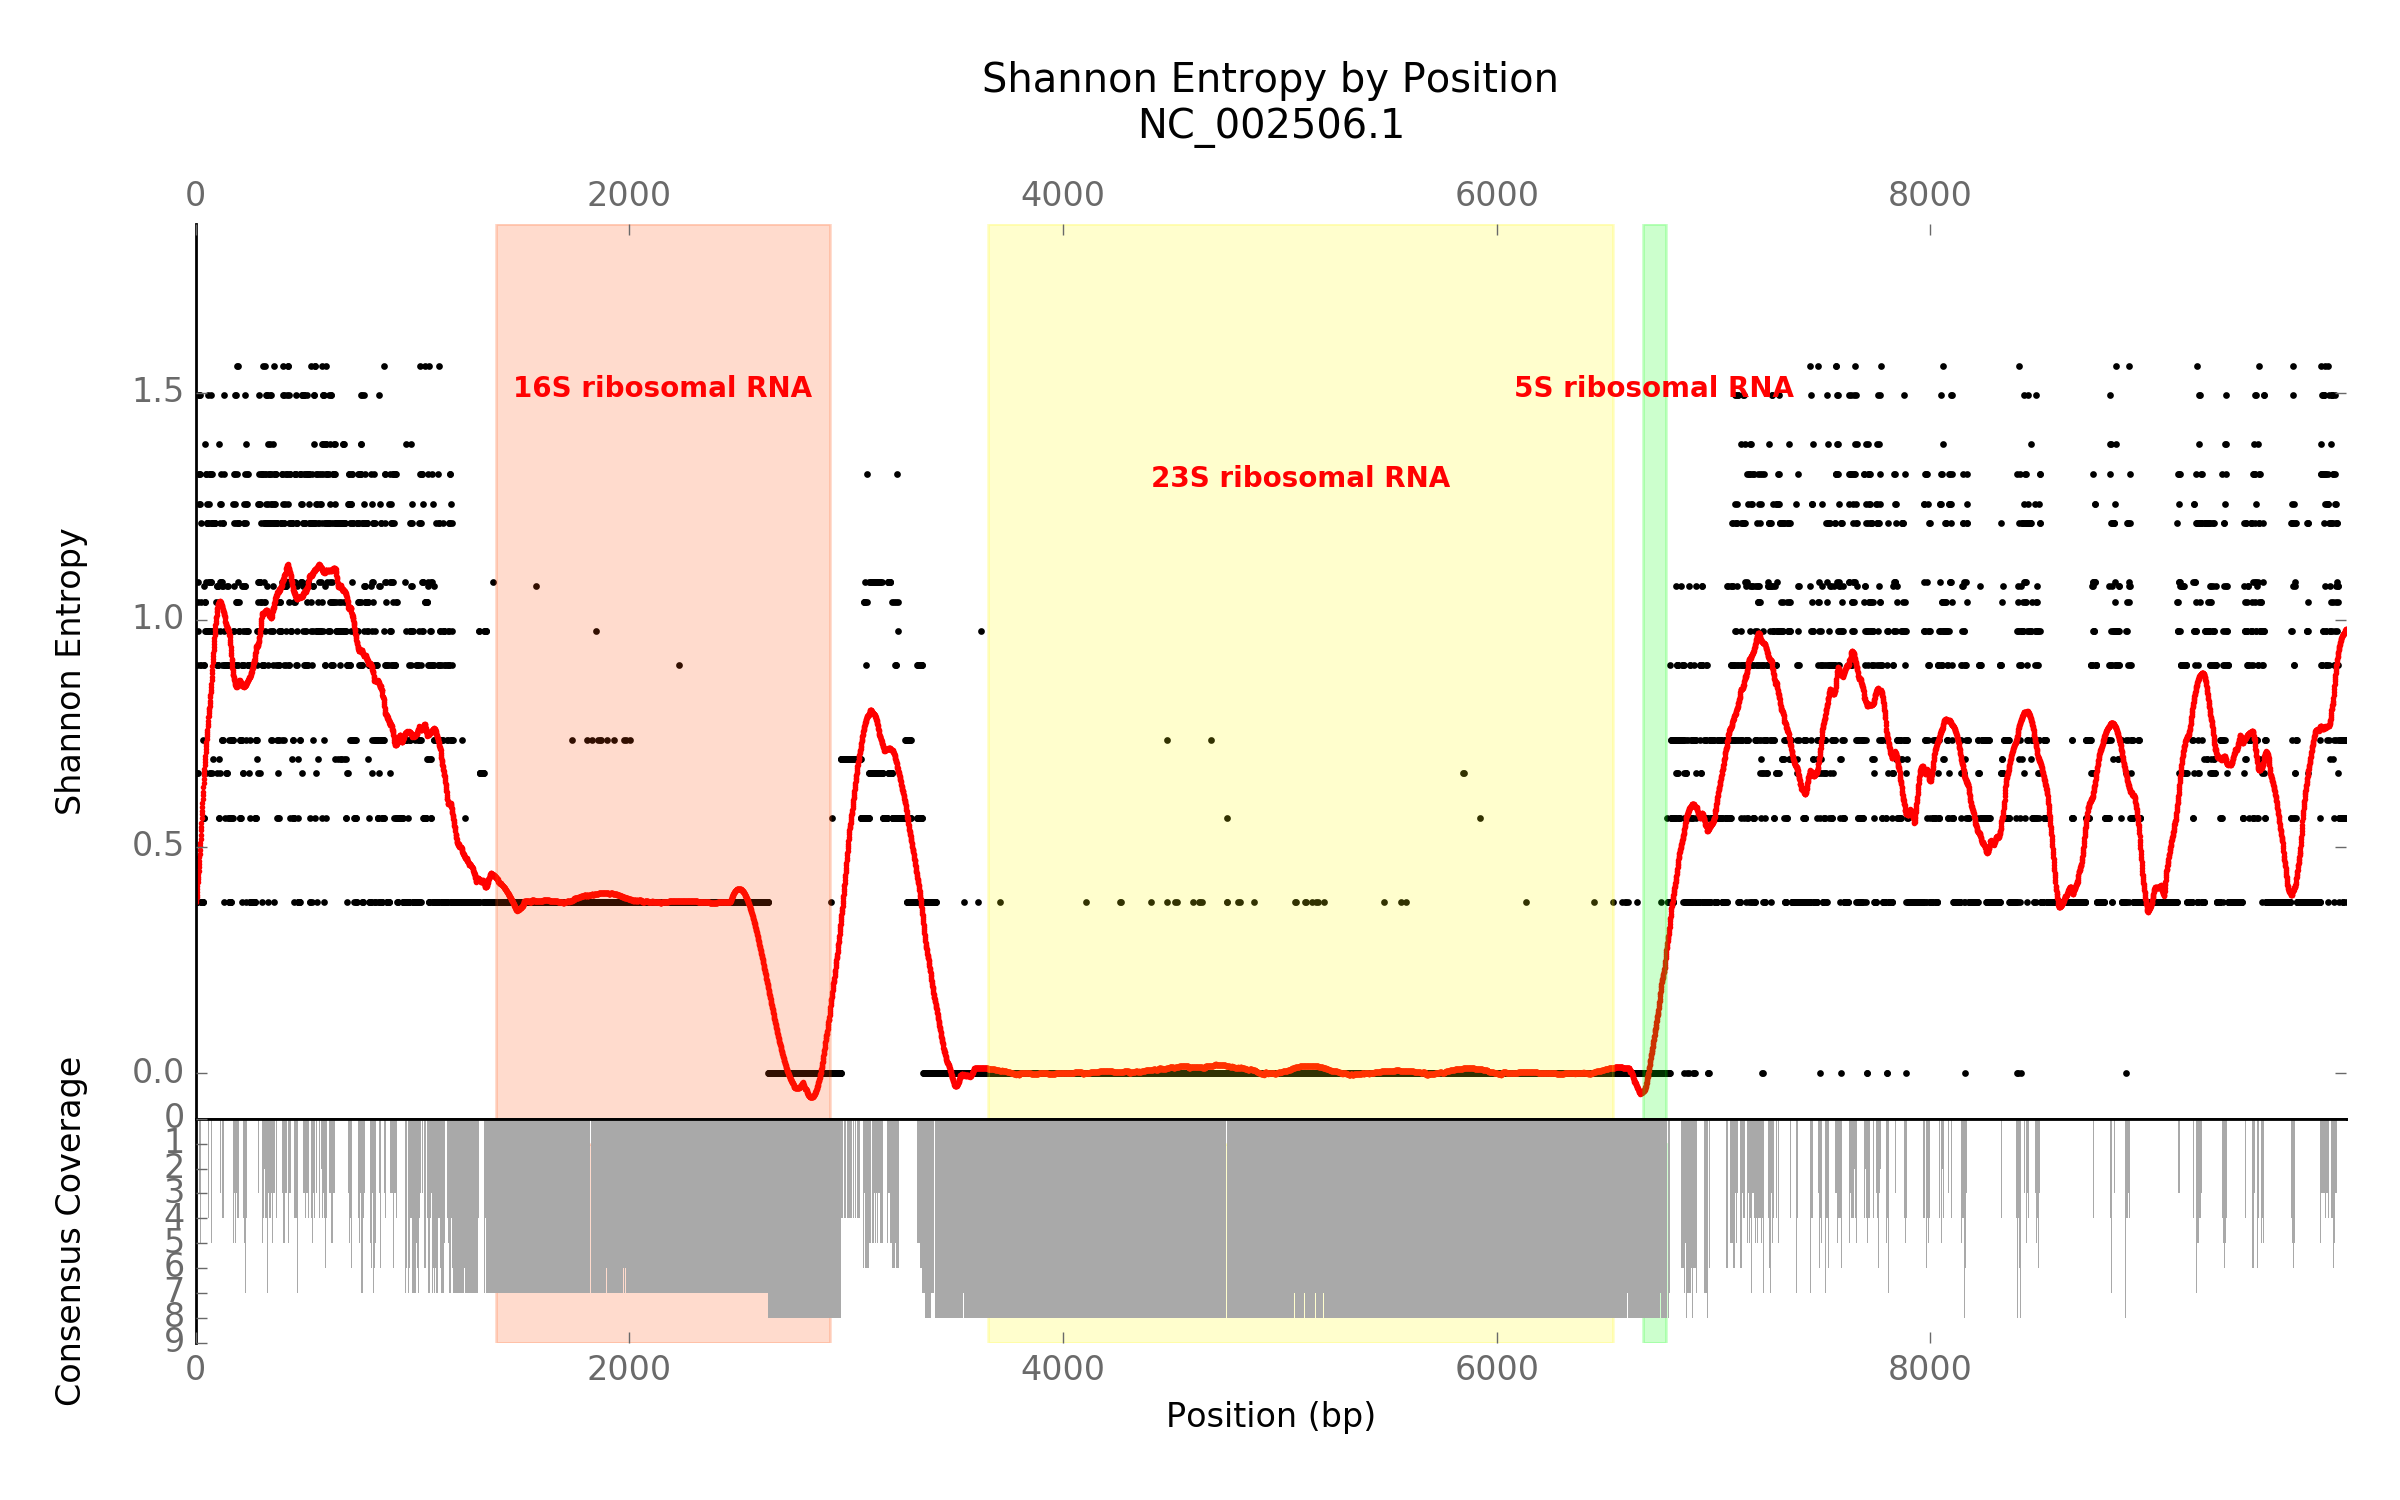
\includegraphics[width=0.95\textwidth]{gage_entropy_figures/NC_002506.1_entropy_plot}
    \caption{\textit{V. cholerae El Tor str. N16961} (NC\_002505.1) (NC\_002506.1)}
    \label{fig:ent_vib}
  \end{subfigure}
  \begin{subfigure}[b]{.45\textwidth}
    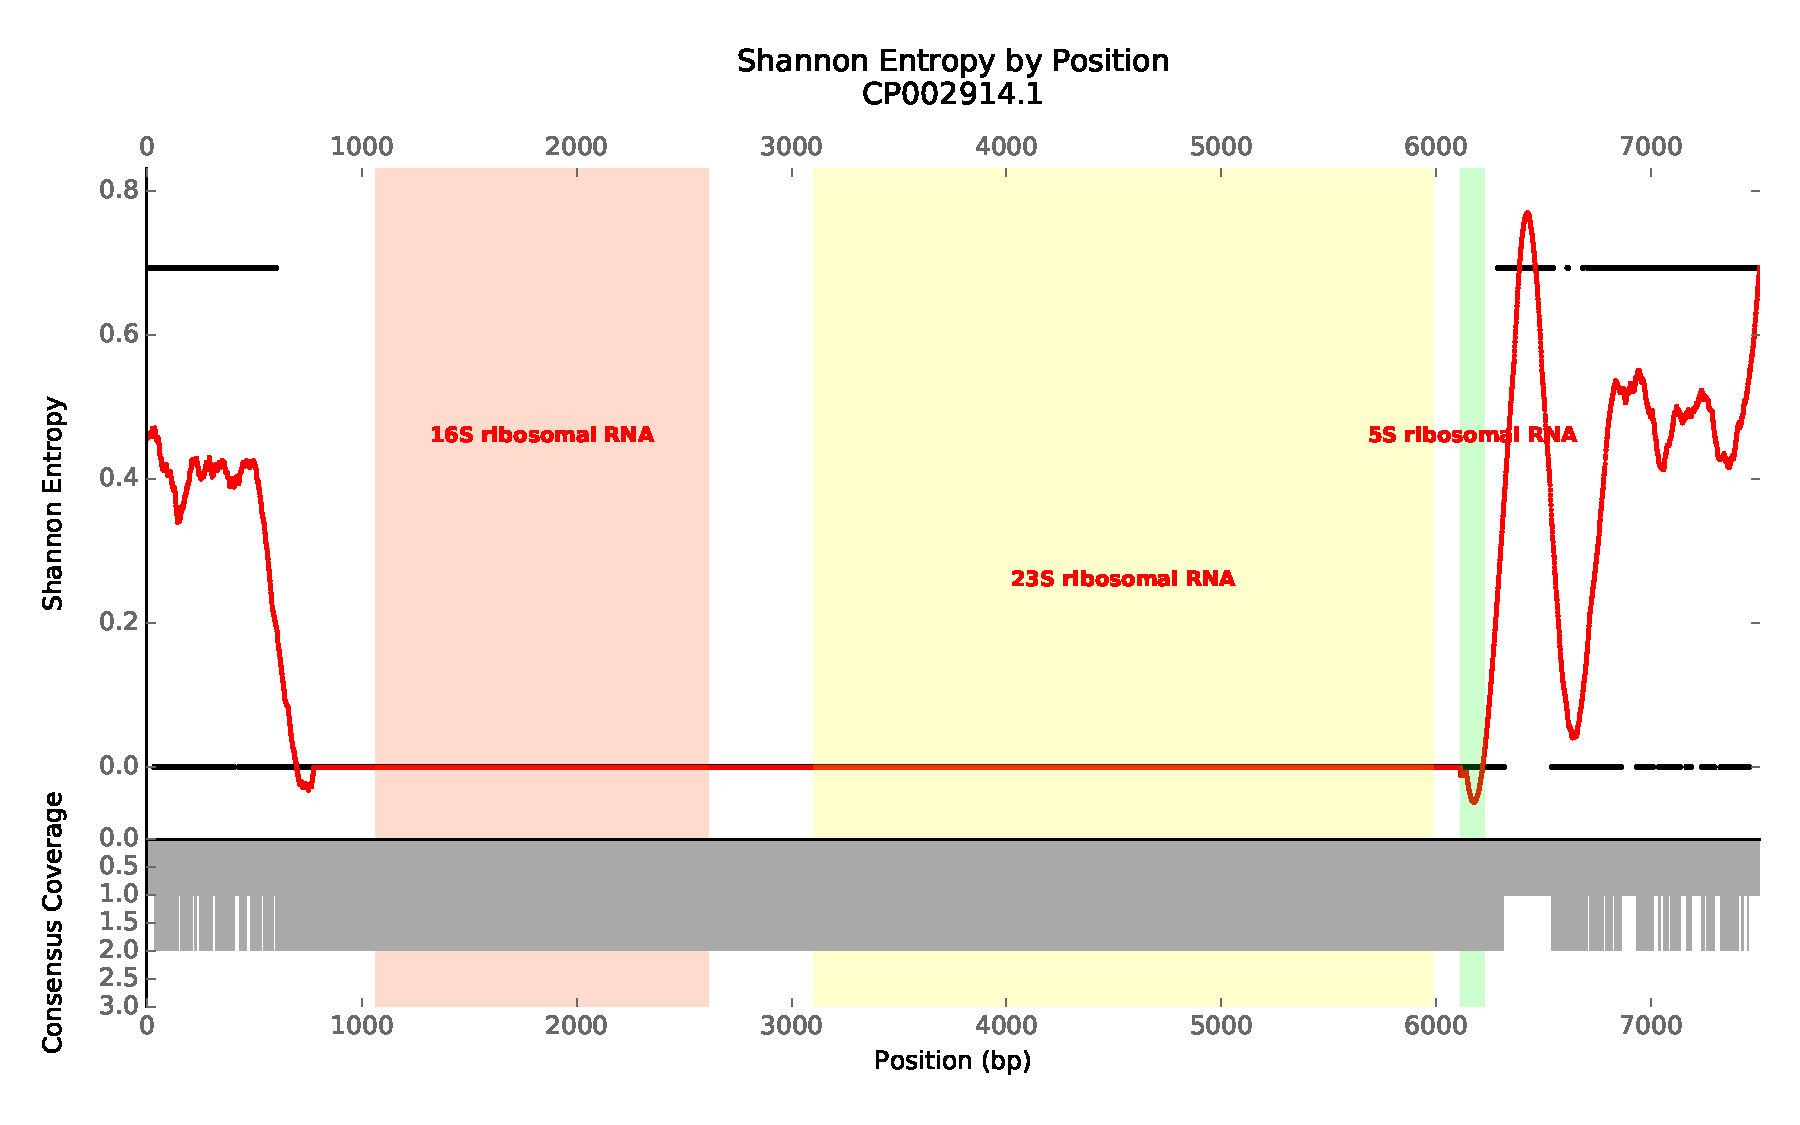
\includegraphics[width=0.95\textwidth]{gage_entropy_figures/CP002914.1_entropy_plot}
    \caption{\textit{X. axonopodis pv. Citrumelo} (CP002914.1)}
  \end{subfigure}
  \caption{riboScan.py,riboSelect.py, and riboSnag.py were run on all the genomes used as references for \textit{de fere novo} assemblies. Consensus alignment depth (grey bars) and Shannon entropy (black points, smoothed entropy as red line) for aligned rDNA regions.}
  \label{fig:ent_gage}

\end{figure}
